%  LaTeX support: latex@mdpi.com 
%  For support, please attach all files needed for compiling as well as the log file, and specify your operating system, LaTeX version, and LaTeX editor.

%=================================================================
\documentclass[sensors,article,submit,moreauthors]{Definitions/mdpi} 
%\documentclass[journal,article,submit,moreauthors,unicode]{Definitions/mdpi} % For some letters Palatino lacks
%\documentclass[preprints,article,submit,moreauthors]{Definitions/mdpi} 
%\documentclass[preprints,article,submit,moreauthors,unicode]{Definitions/mdpi} 
% For posting an early version of this manuscript as a preprint, you may use "preprints" as the journal. Changing "submit" to "accept" before posting will remove line numbers.

%--------------------
% Class Options:
%--------------------
%----------
% journal
%----------
% Choose between the following MDPI journals:
% aam, aamr, aapm, acbr, accountaudit, acn, acoustics, actuators, addictions, addictprev, adhesives, adolescents, aee, aep, aerobiology, aeronautics, aerospace, agriculture, agriengineering, agrochemicals, agronomy, ai, aiaerosp, aiagents, aibiol, aichem, aieng, aimater, aimed, aipa, air, aisens, aisoc, aiua, algorithms, allergies, alloys, amh, analog, analytica, analytics, anatomia, anesthres, animals, antibiotics, antibodies, antioxidants, applbiosci, appliedchem, appliedmath, appliedphys, applmech, applmicrobiol, applnano, applsci, aps, aquacj, archaeolstud, architecture, arm, arthropoda, asc, asd, asi, astronautics, astronomy, atmosphere, atoms, audiolres, automation, axioms, bacteria, batteries, bcrc, bdcc, beverages, bioactives, biochem, bioengineering, biologics, biology, biomass, biomechanics, biomed, biomedicines, biomedinformatics, biomimetics, biomolecules, biophysica, bioresourbioprod, biosensors, biosphere, biotech, birds, blockchains, bloods, blsf, brainsci, breath, bse, buildings, cancers, carbon, cardio, cardiogenetics, cardiovascmed, catalysts, cdr, cells, ceramics, challenges, chemeco, chemengineering, chemistry, chemosensors, chemproc, children, chips, cimb, civileng, cleantechnol, climate, clinbioenerg, clinpract, clockssleep, cmd, cmtr, coasts, coatings, colloids, colorants, complexities, complications, compounds, computation, computers, condensedmatter, conservation, constrmater, cosmetics, covid, crops, cryo, cryptography, crystals, csmf, ctn, culture, curroncol, cyber, dairy, data, ddc, dentistry, dermato, dermatopathology, designs, devices, dgg, dhi, diabetology, diagnostics, dietetics, digital, disabilities, diseases, diversity, dna, drones, drugreact, drylandsci, dynamics, earth, ebj, ece, ecm, eco-environsci, ecologies, edm, eesp, electricity, electrochem, electronicmat, electronics, embodiedintell, encyclopedia, endocrines, energies, eng, engproc, entomology, entropy, environments, environremediat, enzymology, epidemiologia, epigenomes, epilepsy, esa, est, fermentation, fibers, fintech, fire, fishes, fluids, foodeng, foods, forecasting, forensicsci, forests, fossstud, foundations, fractalfract, freshwater, fuels, future, futureinternet, futurepharmacol, futurephys, futuretransp, galaxies, gases, gastroent, gastrointestdisord, gastronomy, gels, genes, geochem, geographies, geohazards, geomatics, geometry, geosciences, geotechnics, geriatrics, germs, glacies, grainsci, grasses, green, greenhealth, gucdd, gynecolcancer, hardware, hazardousmatters, healthcare, healthcmater, hearts, hemato, hematolrep, hep, heritage, higheredu, highthroughput, hls, horticulturae, hospitals, humanoids, hydrobiology, hydrogen, hydrology, hydrometeorology, hydropower, hygiene, idhm, idr, iic, ijem, ijerph, ijgi, ijmd, ijms, ijns, ijom, ijp, ijpb, ijt, ijtm, ijtpp, ijtst, ime, immuno, industries, inflammj, informatics, information, infrastructures, inorganics, insects, instruments, inventions, iot, iron, j, jaestheticmed, jal, japma, jcdd, jcm, jcp, jcrm, jcs, jcto, jdad, jdb, jdcp, jdream, jemr, jeta, jfb, jfmk, jfth, jgbg, jgg, jimaging, jissn, jlpea, jmahp, jmmp, jmms, jmp, jmse, jne, jnt, jof, joitmc, joma, jop, joptm, jor, jox, jpbi, jphytomed, jpm, jsan, jtaer, jvd, jzbg, kidneydial, kinasesphosphatases, knowledge, labmed, laboratories, lam, land, langtechnol, lasers, legumes, life, lights, limnolrev, lipidology, liquids, livers, logics, logistics, lubricants, lymphatics, machines, macromol, magnetism, magnetochemistry, make, marinedrugs, maritime, materials, materproc, mathematics, mca, mcb, measurements, meb, medicina, medicines, medsci, membranes, merits, metabolites, metals, metamaterialsadv, meteorology, methane, metrics, metrology, micro, microarrays, microbiolres, microchem, microelectronics, micromachines, microorganisms, microplastics, microwave, minerals, mining, mmphys, modelling, molbank, molecules, mollusca, mps, msf, mti, multimedia, muscles, musculoskeletsci, mutation, nanoenergyadv, nanomanufacturing, nanomaterials, ncrna, ndt, network, neuroglia, neuroimaging, neurolint, neurosci, nitrogen, numbertheory, nursrep, nutraceuticals, nutrients, obesities, occuphealth, oceans, ohbm, onco, optics, optoelectronics, oral, organics, organoids, osteology, oxygen, pandemics, parasites, parasitologia, particles, pathogens, pathophysiology, pediatrrep, pets, pharmaceuticals, pharmaceutics, pharmacoepidemiology, pharmacy, phc, philosophies, photochem, photonics, photovoltaics, phycology, physchem, physics, physiologia, pjm, plants, plasma, platforms, pnr, pollutants, polymers, polysaccharides, populations, poultry, powders, ppi, precision, precisoncol, prevhealthc, proceedings, processes, prosthesis, proteomes, psf, psychiatryint, psychoactives, purification, quantumrep, quaternary, qubs, radiation, rareearths, rdt, reactions, realestate, receptors, recycling, regeneration, remotesensing, reports, reprodmed, resources, rheumato, rjpm, robotics, rsee, ruminants, safety, sanpp, sca, sci, scipharm, sclerosis, seeds, sensors, senssyst, separations, sexes, sgf, shi, signals, sinusitis, siuj, skins, smartcities, smartfish, smartgrids, sna, societies, software, soilsystems, solar, solids, spectroscj, sports, standards, stats, std, sti, stomatology, stratsediment, stresses, strokerep, superintelligence, surfaces, surgeries, susagric, suschem, susenvmgmt, sustainability, sustainfoods, sustainpackag, symmetry, synbio, systems, tae, targets, taxonomy, technologies, telecom, test, textiles, thalassrep, therapeutics, thermo, timespace, tomography, totalenviron, toxics, toxins, tph, transplantology, transportation, traumacare, traumas, treeres, tri, tropicalmed, universe, urbansci, uro, vaccines, vehicles, veinslymphat, venereology, vetsci, vibration, virtualworlds, viruses, vision, vsd, waste, water, welding, wem, wetlres, wevj, wild, wind, winestud, women, world, xscience, zoonoticdis, zoos

%---------
% article
%---------
% The default type of manuscript is "article", but can be replaced by: 
% abstract, addendum, article, benchmark, book, bookreview, briefcommunication, briefreport, casereport, changes, clinicopathologicalchallenge, comment, commentary, communication, conceptpaper, conferenceproceedings, correction, conferencereport, creative, datadescriptor, discussion, entry, expressionofconcern, extendedabstract, editorial, essay, erratum, fieldguide, hypothesis, interestingimages, letter, meetingreport, monograph, newbookreceived, obituary, opinion, proceedingpaper, projectreport, reply, retraction, review, perspective, protocol, shortnote, studyprotocol, supfile, systematicreview, technicalnote, viewpoint, guidelines, registeredreport, tutorial, giantsinurology, urologyaroundtheworld, patentsummary

% supfile = supplementary materials

%----------
% submit
%----------
% The class option "submit" will be changed to "accept" by the Editorial Office when the paper is accepted. This will only make changes to the frontpage (e.g., the logo of the journal will get visible), the headings, and the copyright information. Also, line numbering will be removed. Journal info and pagination for accepted papers will also be assigned by the Editorial Office.

%------------------
% moreauthors
%------------------
% If there is only one author the class option oneauthor should be used. Otherwise use the class option moreauthors.

%=================================================================
% MDPI internal commands - do not modify
\firstpage{1} 
\makeatletter 
\setcounter{page}{\@firstpage} 
\makeatother
\pubvolume{1}
\issuenum{1}
\articlenumber{0}
\pubyear{2026}
\copyrightyear{2026}
%\externaleditor{Firstname Lastname} % More than 1 editor, please add `` and '' before the last editor name
\datereceived{ } 
\daterevised{ } % Comment out if no revised date
\dateaccepted{ } 
\datepublished{ } 
%\datecorrected{} % For corrected papers: "Corrected: XXX" date in the original paper.
%\dateretracted{} % For retracted papers: "Retracted: XXX" date in the original paper.
%\doinum{} % Used for some special journals, like molbank
%\pdfoutput=1 % Uncommented for upload to arXiv.org
%\CorrStatement{yes}  % For updates
%\longauthorlist{yes} % For many authors that exceed the left citation part
%\IsAssociation{yes} % For association journals

%=================================================================
% Add packages and commands here. The following packages are loaded in our class file: fontenc, inputenc, calc, indentfirst, fancyhdr, graphicx, epstopdf, lastpage, ifthen, float, amsmath, amssymb, lineno, setspace, enumitem, mathpazo, booktabs, titlesec, etoolbox, tabto, xcolor, colortbl, soul, multirow, microtype, tikz, totcount, changepage, attrib, upgreek, array, tabularx, pbox, ragged2e, tocloft, marginnote, marginfix, enotez, amsthm, natbib, hyperref, cleveref, scrextend, url, geometry, newfloat, caption, draftwatermark, seqsplit
% cleveref: load \crefname definitions after \begin{document}

%=================================================================
% Please use the following mathematics environments: Theorem, Lemma, Corollary, Proposition, Characterization, Property, Problem, Example, ExamplesandDefinitions, Hypothesis, Remark, Definition, Notation, Assumption
%% For proofs, please use the proof environment (the amsthm package is loaded by the MDPI class).

%=================================================================
% Drafting helpers (remove before submission)
\newcommand{\todo}[1]{\textcolor{red}{[\textbf{TODO:} #1]}}

%=================================================================
\Title{Protective-Field Barrier Functions: LiDAR-Based Safety Filtering for Learned Navigation of Industrial Mobile Robots}

\newcommand{\orcidauthorA}{0000-0000-0000-000X} % TODO: Mahdi's ORCID

\Author{Mahdi Kahoul $^{1,}$*\orcidA{} and \todo{Supervisor Name} $^{1}$}

\AuthorNames{Mahdi Kahoul and \todo{Supervisor Name}}

\address{%
$^{1}$ \quad \todo{Laboratory / Department}, University of Biskra, Biskra, Algeria; mahdi.kahoul@univ-biskra.dz}

\corres{Correspondence: mahdi.kahoul@univ-biskra.dz}

% Abstract (draft; results sentences are placeholders until evaluation)
\abstract{Autonomous mobile robots in industrial facilities share their workspace with people and are protected by certified safety laser scanners that halt the vehicle whenever an obstacle enters a speed-dependent protective field. Learning-based local planners combined with control barrier function (CBF) safety filters are typically evaluated by their collision rate, a quantity the certified layer already bounds, while the protective stops that interrupt operation remain unmeasured. This paper proposes the Protective-Field Barrier (PFB), a LiDAR-based CBF safety filter whose safe set is the complement of the certified safety function's own trigger set: a footprint-aware, speed-, direction- and rotation-dependent protective field evaluated on every scanner sector. The filter is placed between a Soft Actor-Critic local planner, trained with the filter in the loop and without proximity reward shaping, and an emulated certified safety layer that remains active beneath every controller. The approach is evaluated on a holonomic mecanum platform in procedurally generated warehouse layouts containing obstacles absent from the map, against classical and learned baselines, under a preregistered protocol with protective stops per 100 m as the primary endpoint. \todo{Results: one or two sentences with the main effect sizes and confidence intervals.} \todo{Conclusion: one sentence.}}

\keyword{control barrier functions; safety filter; safety laser scanner; protective field; LiDAR; deep reinforcement learning; soft actor-critic; autonomous mobile robots; Industry 4.0}

%%%%%%%%%%%%%%%%%%%%%%%%%%%%%%%%%%%%%%%%%%
\begin{document}

%%%%%%%%%%%%%%%%%%%%%%%%%%%%%%%%%%%%%%%%%%
\section{Introduction}

Autonomous mobile robots (AMRs) are replacing fixed conveyors and manually driven vehicles as the means of moving material through factories and warehouses in Industry~4.0 facilities. Unlike classical automated guided vehicles, which follow fixed routes, AMRs plan their own paths and share aisles, intersections and workstations with human workers. Their safety in such shared spaces does not rest on the navigation software. It is provided by a certified safety function, built around safety laser scanners that monitor a protective field around the vehicle and command a stop whenever an object enters it~\citep{iso3691-4,iec61496-3}. Because the stopping distance grows with speed, the field is not fixed: integrators configure several field sets and switch between them according to the vehicle's speed and direction of travel, and the switching itself is a safety function that must reach a required performance level~\citep{iso3691-4,iso13849-1}. A protective stop latches until the field is clear and the restart conditions are met. Every stop therefore interrupts a transport task, and frequent stops directly reduce throughput.

Deep reinforcement learning (DRL) has become a widely studied approach to the local planning problem, in which a policy maps sensor observations, typically from a 2D LiDAR, to velocity commands~\citep{le2024review,he2021review}. Off-policy actor--critic methods such as Soft Actor-Critic (SAC)~\citep{haarnoja2018sac} and TD3~\citep{fujimoto2018td3} handle the continuous action spaces of mobile bases, and hierarchical architectures, in which a classical global planner supplies waypoints to a learned local policy, have been reported to outperform both purely classical and end-to-end learned navigation~\citep{zhu2023hierarchical,kolomeytsev2025hybrid,zhao2025hierarchical}. In most of this work, however, safety is expressed through the reward: collisions are penalised and proximity to obstacles is discouraged by shaping terms~\citep{taheri2024ppo,cai2025agv}. Such policies avoid obstacles statistically rather than by construction, and the proximity terms compete with the task itself. A preliminary study by the authors on the platform used here observed that a SAC local planner trained in this way degraded markedly in tight passages, where reaching the goal requires precisely the close approaches that the reward discourages. The present study tests that diagnosis directly.

Control barrier functions (CBFs) offer a principled alternative~\citep{ames2017cbfqp,ames2019cbf}. A CBF defines a safe set through a function of the state and constrains the control input so that the set is forward invariant; in its most common use, a small quadratic program (QP) minimally modifies a nominal command, such as the output of a learned policy, whenever that command would violate the barrier condition. CBF safety filters have been combined with learned motion planners~\citep{wang2022ensuring} and with DRL navigation policies in several forms: as a runtime filter on a learned policy~\citep{guo2025radar}, with a learned adaptation of the barrier's parameters~\citep{mohammad2025sacadapt,mohammad2025corridor}, and as a filter applied during training so that the policy internalises the constraint~\citep{cheng2019endtoend,yang2025cbfrl}.

Two features of this body of work limit its relevance to industrial deployment. First, safety is evaluated as a collision rate in simulation, in a world that contains no safety hardware. On a certified AMR, collisions with obstacles inside the scanner plane are already prevented by the certified layer, whatever the planner does, and a software filter acting on a neural policy will not replace that layer, since it is not itself a certified safety function. The operational cost that remains is the protective stop. Second, the safe sets used by LiDAR-based barriers are typically defined by distances to points or obstacles. None of them takes the shape of the protective field that the safety hardware actually monitors: deeper in the direction of travel, growing with speed, tied to the vehicle's footprint, and swept by the vehicle's rotation during the stopping manoeuvre. A filter that keeps obstacles at a fixed distance may still let them into the protective field and trigger a stop; a filter that is too conservative may stop the robot by itself.

This paper addresses the resulting question: \emph{can a barrier function constructed from the geometry of industrial protective fields allow a learned local planner to pass tight and cluttered spaces while triggering fewer protective stops, and at what cost in task completion and mission time?} The contributions are as follows.
\begin{itemize}
\item \textbf{The Protective-Field Barrier (PFB).} We formulate a LiDAR-sector CBF safety filter whose safe set is the complement of the certified safety function's own trigger set. The barrier is defined per scanner sector from the measured range, the robot's footprint along that bearing, and a field depth that accounts for the motion reachable within the response time and for the rotation swept during braking, on a holonomic platform. The filter is solved as a QP with the mecanum wheel-speed limits as constraints.
\item \textbf{Learning with safety outside the reward.} We train a SAC local planner with the PFB in the training loop and without proximity shaping, so that the reward expresses only the transport task, and compare it with shaped, constrained (Lagrangian) and post-hoc-filtered alternatives.
\item \textbf{An evaluation that includes the certified layer.} We place an emulated certified safety layer, with speed-banded protective fields and latched stops, beneath every controller, learned and classical, and adopt protective stops per 100\,m as the primary endpoint, on procedurally generated warehouse layouts in which obstacles absent from the map are placed near the planned route.
\item \textbf{A verified and preregistered protocol.} Hypotheses, comparators, test scenarios and the statistical analysis, a seed-aware bootstrap of rate ratios, were fixed before evaluation. We also report the simulation and sensing defects that verification uncovered before training, including a sensor blind zone inside the protective field and load-dependent scan corruption, because each would have biased a safety evaluation silently.
\end{itemize}

The remainder of the paper is organised as follows. Section~\ref{sec:related} reviews related work. Section~\ref{sec:system} describes the platform, sensing and the certified-layer emulator. Section~\ref{sec:pfb} formulates the PFB and the learning design. Section~\ref{sec:design} presents the experimental design. Section~\ref{sec:results} reports the results, Section~\ref{sec:discussion} discusses them and their limitations, and Section~\ref{sec:conclusions} concludes.

%%%%%%%%%%%%%%%%%%%%%%%%%%%%%%%%%%%%%%%%%%
\section{Related Work}\label{sec:related}

\subsection{Deep Reinforcement Learning for Local Planning}

Value-based methods first demonstrated DRL on high-dimensional control problems~\citep{mnih2015dqn}, and continuous-control actor--critic algorithms, from DDPG~\citep{lillicrap2016ddpg} to TD3~\citep{fujimoto2018td3} and SAC~\citep{haarnoja2018sac}, made the approach practical for velocity commands on mobile bases; PPO~\citep{schulman2017ppo} is preferred where many parallel simulations are available. Reviews of DRL navigation identify 2D LiDAR, compressed into angular sectors, as the dominant observation for its compactness and transferability~\citep{le2024review,liu2024sac}. The classical baseline for reactive local planning remains the Dynamic Window Approach~\citep{fox1997dwa}, which samples admissible velocities and scores them against a hand-tuned cost.

Hierarchical designs combine a global planner on a map with a learned local policy that follows waypoints on the global path. This structure reduces the difficulty of the learning problem and improves sample efficiency and generalisation~\citep{zhu2023hierarchical}; variants pair graph-based global planners with SAC~\citep{kolomeytsev2025hybrid}, use metaheuristic global planning~\citep{zhao2025hierarchical}, or learn when to replan~\citep{honda2024replan}. The robot's geometry is usually simplified: most learned local planners assume differential-drive kinematics, and those that handle explicit footprints address rectangular differential-drive robots~\citep{zhang2025drldclp}. Holonomic platforms with mecanum wheels, whose action space includes lateral velocity and whose wheels slip, are rarely treated. Simulation-trained policies also face a reality gap, addressed through domain randomisation and curricula~\citep{zhao2020sim2real}. Finally, evaluation practice in the field varies: results from single training seeds are common despite the large variance between seeds that DRL is known to exhibit~\citep{henderson2018matters,agarwal2021precipice,cancelliere2025eval}.

\subsection{Safety in Learned Navigation}

Three families of methods address safety in reinforcement learning. The first, and the most common in navigation, encodes safety in the reward through collision penalties and proximity shaping~\citep{taheri2024ppo,cai2025agv,li2024warehouse}. It offers no guarantee and couples the safety objective to the task objective. The second treats safety as a constraint on expected cost within a constrained Markov decision process~\citep{altman1999cmdp}, solved with Lagrangian relaxation or trust-region methods~\citep{achiam2017cpo}; constraints are then satisfied in expectation over training, not at every step. The third enforces safety at run time by modifying unsafe actions, either through a shield derived from a formal specification~\citep{alshiekh2018shielding} or through a control-theoretic safety filter. The present work belongs to the third family but compares against the first two: the shaped SAC and SAC-Lagrangian baselines represent them directly.

\subsection{Control Barrier Function Safety Filters}

For a control-affine system $\dot{x} = f(x) + g(x)u$ and a safe set $\mathcal{C} = \{x : h(x) \geq 0\}$, the CBF condition $\dot{h}(x,u) \geq -\alpha(h(x))$, with $\alpha$ an extended class-$\mathcal{K}$ function, renders $\mathcal{C}$ forward invariant~\citep{ames2017cbfqp,ames2019cbf}. Because the condition is affine in $u$, the safe input closest to a nominal command is the solution of a QP that can be solved at control rates. This makes CBFs a natural safety filter for learned controllers. Barrier-based filters have been used to ensure the safety of learning-based motion planners~\citep{wang2022ensuring}, and constructed at run time from the policy itself to obtain robust filters~\citep{knoedler2025onthefly}.

In DRL navigation specifically, a PPO policy has been combined with a CBF-QP filter on an omnidirectional robot in simulation~\citep{guo2025radar}; a SAC policy has been trained to adapt the barrier's class-$\mathcal{K}$ gain online, so that the filter is neither too conservative nor too permissive, and validated on a real robot~\citep{mohammad2025sacadapt}, and extended to corridor-shaped safe sets within model predictive contouring control~\citep{mohammad2025corridor}. Barriers have also been encoded in the cost of an optimal control problem solved by actor--critic updates~\citep{wang2024safeadp}, and learned barriers have been integrated with a fleet-management framework for warehouse navigation among pedestrians~\citep{farrell2025warehouse}. Applying the filter during training, so that the policy learns from filtered roll-outs and internalises the constraint, has been shown to improve safety and allow deployment without a run-time filter~\citep{cheng2019endtoend,yang2025cbfrl}. The present work also trains with the filter in the loop, but keeps the filter at deployment and evaluates it against an industrial safety layer rather than in isolation.

\subsection{Barriers from Range Sensing}

Implementing a CBF on a real robot requires the safe set to be constructed from sensor data rather than from known obstacle models. Occupancy-grid barriers address the limited field of view of LiDAR by retaining obstacles that have left the sensor's view~\citep{raja2024ogmcbf}, a reminder that unobserved space must not be treated as free. Barriers that account for the relative velocity between humans and mobile robots have been proposed to anticipate fast approaches in shared workspaces~\citep{zeng2025relvel}. In these formulations the safe set is defined by distances, possibly velocity-dependent, to observed points or obstacles; the robot's footprint and the geometry of its stopping manoeuvre enter only through margins.

\subsection{Industrial Safety Standards and Protective Fields}

Industrial driverless vehicles are governed by ISO~3691-4~\citep{iso3691-4}, under which personnel detection is typically achieved with safety laser scanners qualified as active opto-electronic protective devices~\citep{iec61496-3}. The protective field must contain the vehicle's stopping travel from the moment of detection, so its size depends on speed, and field switching by speed and direction is itself a safety function implemented in the certified safety controller~\citep{iso13849-1}. Barrier functions derived from safety-standard stopping requirements have recently been proposed for collaborative manipulators, predicting the minimum human--robot separation during a worst-case stop~\citep{iso10218cbf2026}. To our knowledge, no comparable construction exists for mobile bases, and no study of learned navigation models the certified layer beneath the controller or reports protective stops.

\subsection{Positioning}

Table~\ref{tab:positioning} summarises the closest works along the dimensions that define this study.

\begin{table}[H]
\caption{Positioning of this work against the closest related studies. \todo{verify every cell against the original papers before submission.}\label{tab:positioning}}
\begin{adjustwidth}{-\extralength}{0cm}
\newcolumntype{L}{>{\raggedright\arraybackslash}X}
\begin{tabularx}{\fulllength}{p{3.6cm}LLLL}
\toprule
\textbf{Work} & \textbf{Learned component} & \textbf{Safety mechanism} & \textbf{Safe set} & \textbf{Safety evaluated as} \\
\midrule
Guo et al.~\citep{guo2025radar} & PPO navigation policy & Runtime CBF-QP filter & Distance to obstacles & Collision avoidance, task success \\
Mohammad and Bezzo~\citep{mohammad2025sacadapt} & SAC adapts the barrier gain & Runtime CBF filter & Distance to obstacles & Collisions, deadlocks \\
Yang et al.~\citep{yang2025cbfrl} & RL policy & CBF filter during training only & Task-specific & Safe behaviour without a run-time filter \\
Raja et al.~\citep{raja2024ogmcbf} & None & Runtime CBF filter & Occupancy grid with memory & Safety violations \\
ISO~10218 CBF~\citep{iso10218cbf2026} & None (manipulator) & Standard-derived barrier & Predicted human--robot separation & Separation during worst-case stop \\
\midrule
\textbf{This work} & SAC trained with the filter & Runtime PFB filter above a certified-layer emulator & Complement of the protective-field trigger set & Protective stops per 100\,m, with success and mission time \\
\bottomrule
\end{tabularx}
\end{adjustwidth}
\end{table}

%%%%%%%%%%%%%%%%%%%%%%%%%%%%%%%%%%%%%%%%%%
\section{System and Problem Formulation}\label{sec:system}

Figure~\ref{fig:architecture} shows the system. A global planner supplies a route on a map that omits some obstacles; a local controller, learned or classical, proposes a velocity command; the PFB filters it; an emulated certified safety layer, active beneath every controller, may override any command with a latched protective stop; and the base applies what remains through its kinematic limits. This section describes each component below the controller, and closes with the formal definitions on which the evaluation rests. All quantities are in SI units, in the body frame ($+x$ forward, $+y$ left, bearings in $(-\pi,\pi]$), and every value is the configured one; the notation is collected in Appendix~\ref{app:notation} (Table~\ref{tab:notation}).

\begin{figure}[H]
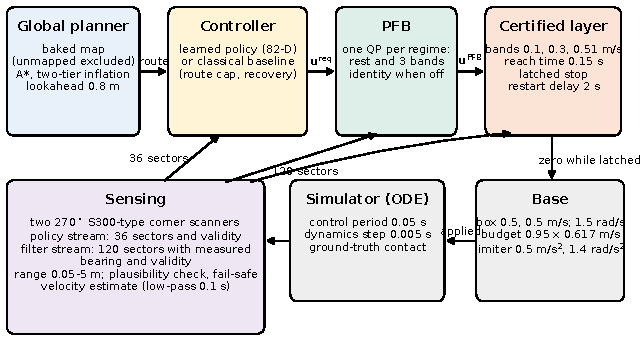
\includegraphics[width=\textwidth]{figures/fig1_architecture.pdf}
\caption{System architecture. Every controller (learned policy or classical baseline) sends its command through the same path: the PFB slot (identity when the filter is off), the certified-layer emulator, which decides on the scan already in hand and may replace the command by zero while a protective stop is latched, and the base's velocity box, wheel-speed budget and acceleration limiter. The policy receives the 36-bin policy stream; the PFB, the certified layer and the classical baselines receive the 120-bin filter stream with its bearings and validity flags. Generated from the configuration by \texttt{paper/figures/scripts/fig1\_architecture.py}.\label{fig:architecture}}
\end{figure}

\subsection{Platform and Actuation}\label{sec:platform}

The platform is a holonomic base derived from the KUKA youBot, with four mecanum wheels, simulated in CoppeliaSim~\citep{rohmer2013vrep} with the ODE physics engine at a dynamics step of 0.005\,s and a control period $\Delta t = 0.05$\,s. The engine is a stated condition of every result: in a pre-registered engine sweep, the same model's heading drift on a 5\,m lateral profile at 0.12\,m/s was 20.55$^\circ$ under Bullet, 0.47$^\circ$ under ODE and 3.12$^\circ$ under Newton, and the run failed under MuJoCo (Appendix~\ref{app:verification}).

\textbf{Footprint.} The robot's outline is the envelope of every shape that can strike an obstacle: the chassis, the wheels and the scanner housings. It is not a datasheet rectangle but a measured footprint table $e(\psi)$, the distance from the body origin to the envelope along each whole-degree bearing, obtained by a collision probe swept in the simulator and interpolated by a periodic spline with a 0.95\,mm margin. Its inscribed and circumscribed radii are $0.20945$\,m and $\rho_{\text{out}} = 0.33742$\,m; the enclosing rectangle has half-length $0.2854$\,m and half-width $0.2086$\,m. Measured values are configured at the upper bound of their measurement bracket, because under-stating a safety footprint is the unsafe direction.

\textbf{Kinematics and wheel-speed budget.} A body command $\mathbf{u} = (v_x, v_y, \omega)$ maps to the wheel speeds through the standard mecanum mixing~\citep{lynch2017modern},
\begin{equation}
\begin{bmatrix}\varpi_{\text{fl}}\\ \varpi_{\text{fr}}\\ \varpi_{\text{rl}}\\ \varpi_{\text{rr}}\end{bmatrix}
= \frac{1}{r_w}
\begin{bmatrix} 1 & -1 & -L\\ 1 & 1 & L\\ 1 & 1 & -L\\ 1 & -1 & L \end{bmatrix}
\begin{bmatrix} v_x\\ v_y\\ \omega\end{bmatrix},
\qquad L = l + w,
\label{eq:mixing}
\end{equation}
% source: pfbnav/sim/robot.py::wheels_from_body (_MIX_SIGNS), per-wheel sign vector omitted
with wheel radius $r_w = 0.05$\,m and lever arm $L = 0.228 + 0.1585 = 0.3865$\,m (half wheelbase plus half track). By Equation~(\ref{eq:mixing}), the fastest wheel's rim speed is $|v_x| + |v_y| + L|\omega|$, and the wheel-speed limit becomes the polytope
\begin{equation}
|v_x| + |v_y| + L\,|\omega| \;\le\; f\,v_{\text{rim}},
\label{eq:budget}
\end{equation}
% source: pfbnav/sim/robot.py::wheel_budget_use, project_to_wheel_budget; configs/base.yaml actuation.wheel_budget
where $v_{\text{rim}} = 0.617$\,m/s is the rim-speed ceiling measured on the saturating diagonal (a torque-balance point, so a load-dependent value) and $f$ is a share of it. The filter's output and the base's final ceiling use $f = 0.95$ ($0.586$\,m/s); a command that exceeds the budget is scaled by one factor in all three components, so its direction and its ratio of turning to translating are preserved. \todo{The configuration and \texttt{robot.py} describe a smaller nominal share, $f = 0.80$, for the controller's command before the filter; no code in the environment applies it. Reported as an inconsistency; text to be settled once resolved.} An axis box $|v_x| \le 0.5$, $|v_y| \le 0.5$\,m/s, $|\omega| \le 1.5$\,rad/s, applied by direction-preserving scaling, sits inside the budget.

\textbf{Acceleration limits as safety-design parameters.} An acceleration limiter bounds every change of the applied command:
\begin{equation}
\big\|(v_x,v_y)_{k} - (v_x,v_y)_{k-1}\big\| \le
\begin{cases} a_{\text{dec}}\,\Delta t & \text{if } \|(v_x,v_y)_{k}\| < \|(v_x,v_y)_{k-1}\|,\\
a_{\max}\,\Delta t & \text{otherwise,}\end{cases}
\qquad |\omega_k - \omega_{k-1}| \le \alpha_{\max}\,\Delta t,
\label{eq:limiter}
\end{equation}
% source: pfbnav/sim/robot.py::limit_acceleration
with the translational step scaled along its own direction, so the limit is isotropic. The values $a_{\max} = 0.5$\,m/s$^2$ and $\alpha_{\max} = 1.4$\,rad/s$^2$ are not measured properties of the youBot. They are \emph{co-specified with the protective fields}: $a_{\max} T$ must be smaller than the narrowest speed band (Section~\ref{sec:emulator}), and $\alpha_{\max}$ is $a_{\max}/\rho_{\text{out}}$ rounded down, so that no point of the body accelerates faster than $a_{\max}$. That the limiter, and not the wheels' torque cap, binds at these values was checked in the simulator. The deceleration bound $a_{\text{dec}} = 1.0$\,m/s$^2$ equals the braking the fields assume, so no controller can command a stop harder than the fields were sized for.

\textbf{Velocity estimate.} The safety layers use the estimated \emph{actual} body velocity $\hat{\mathbf{v}}$, obtained by differencing the pose of the base's reference frame and low-pass filtering it with a time constant of $0.10$\,s. Neither the command, which over-states realised speed under wheel slip, nor wheel odometry, which inherits the same error, is used. The pose is the simulator's ground truth, which a real AMR does not have; this is a stated limitation.

\subsection{Sensing}\label{sec:sensing}

\textbf{Scanner layout.} Two scanners of the SICK S300 type are mounted on diagonally opposite corners of the chassis, each covering 270$^\circ$ with two 135$^\circ$ vision sensors. A rectangle's corner faces 270$^\circ$ of open space, so two opposite-corner scanners see everything outside the outline only if each sees at least 270$^\circ$; the layout was adopted after verification found a blind zone beside the robot with the platform's original centreline 240$^\circ$ pods (Appendix~\ref{app:verification}). The scan plane lies at $0.2206$\,m above the floor, above the wheel tops and the chassis top; obstacles below it are not sensed, and appear as collisions with no protective stop. This is an S300-type layout in simulation; no claim is made that the system uses certified sensing.

\textbf{From pixels to sectors.} Each sensor renders 576 depth pixels across its 135$^\circ$ field of view, a density of 4.27 rays per degree, chosen as the lowest tested density whose range error on a wall at 1--2\,m stays within 10\,mm. The robot itself is rendered, except each sensor's own casing, so the chassis and the other scanner occlude as they would physically; returns that fall inside the footprint plus a 5\,mm margin are the robot and are discarded. The returns of all four sensors are merged into two streams, binned in the simulator and published as one packet per control step:
\begin{itemize}
\item the \emph{policy stream}: 36 sectors of 10$^\circ$, the minimum range in each, with a validity flag;
\item the \emph{filter stream}: 120 sectors of 3$^\circ$, each carrying the minimum range, the bearing at which that range was measured, and a validity flag.
\end{itemize}
Ranges lie in $[0.05, 5.0]$\,m. A sector of the filter stream is denoted $(r_k, \psi_k, \chi_k)$, $k = 1,\dots,120$, with $\chi_k \in \{0,1\}$ its validity. Carrying the measured bearing rather than the sector centre matters to the safety layers, which evaluate a speed- and direction-dependent field at each bearing.

\textbf{Validity and coverage.} A sector is valid only if its whole angular extent, from the footprint edge out to 1.0\,m beyond it, is seen by some sensor \emph{from where that sensor is}, accounting for its field of view and for occlusion by the footprint. Unobserved space is never treated as free: an invalid sector breaches every protective field, and the policy receives validity as a separate channel beside the ranges. The coverage was verified by sweeping a 20\,mm post over a 25\,mm grid from the footprint edge to 1.0\,m beyond it at scan-plane height and classifying each of 7{,}680 cells as observed, flagged invalid, or reported free without observation (a violation). With the corner scanners all 7{,}680 cells were observed on both streams and all 120 filter sectors were valid; with the original centreline pods, 3{,}713 cells were flagged invalid and 60 of 120 filter sectors were valid (Figure~\ref{fig:coverage}).

\begin{figure}[H]
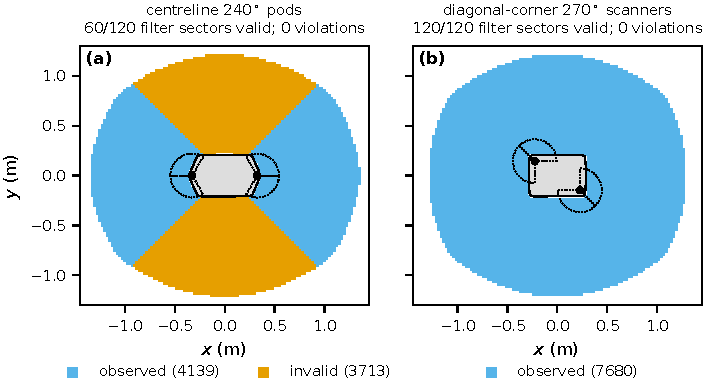
\includegraphics[width=\textwidth]{figures/fig3_coverage.pdf}
\caption{Sensor coverage measured by the dense post sweep (20\,mm post, 25\,mm grid, from the footprint edge to 1.0\,m beyond it, at scan-plane height), filter stream. (\textbf{a}) The platform's original layout, two 240$^\circ$ pods on the centreline: cells beside the robot are flagged invalid, never reported free. (\textbf{b}) The adopted layout, two 270$^\circ$ S300-type scanners on diagonal corners: every cell observed. Sensor positions and fields of view are those recorded by each run. Data: \texttt{runs/diag/COVMAP-centreline\_20260922T163600Z\_seed0} and \texttt{COVMAP-s300\_corners\_20260922T214324Z\_seed0}; script \texttt{paper/figures/scripts/fig3\_coverage.py}.\label{fig:coverage}}
\end{figure}

\textbf{Scan plausibility.} Under heavy CPU load the simulator's renderer was found to deliver occasional corrupted frames: most sectors empty and phantom returns near the scanner corners, in fresh packets that passed the staleness check (Appendix~\ref{app:verification}). Every packet is therefore checked against the last accepted one. A sector is implausible if its range lies outside the interval spanned by the last accepted scan's sectors within $\pm 2$ of it, widened by $\pm 0.06$\,m, both bounds growing with each step since that scan; six or more implausible sectors make the packet corrupt. A corrupt packet is re-rendered up to twice within the same simulation tick; if it is still corrupt, every sector of that step is marked unobserved, which is a fail-safe stop. Such steps are counted as scan faults, and a stop decided on a fail-safed packet is a \emph{scan-fault stop} (Section~\ref{sec:definitions}).

\subsection{The Certified-Layer Emulator}\label{sec:emulator}

The certified layer is emulated as an industrial safety laser scanner with switchable field sets, together with the safety controller that selects the set from the vehicle's speed and direction and latches stops. It is implemented independently of the PFB and runs beneath every controller. It emulates the behaviour of such a system; it does not claim functional-safety compliance. Appendix~\ref{app:realism} compares each of its features with industrial practice.

\textbf{Containment.} The field in force when a stop triggers must contain everything the footprint sweeps from the trigger until the robot is at rest. After a breach, the command still passes during the response time $t_r = 0.10$\,s, and the limiter lets it keep growing. The fields are sized over a \emph{reach time} that adds one control step to the response time,
\begin{equation}
T = t_r + \Delta t = 0.15\ \text{s},
\label{eq:reachtime}
\end{equation}
% source: pfbnav/world/strata.py::certified_params_from_config (reach_time); pfbnav/safety/pfb_field.py::field_params_from_config
and the fields contain the motion reachable within $T$ followed by braking at $a_b = 1.0$\,m/s$^2$ in translation and $\alpha_{\max}$ in rotation.

\textbf{Speed bands.} The field set is selected by the \emph{reachable} speed. With $s$ the composed planar speed (defined below),
\begin{equation}
\bar{v}(s) = \max\!\big(s,\ \min(s + a_{\max}T,\ v_{\text{cap}})\big),
\qquad
\ell(s) = \min\{\ell : \bar{v}(s) \le V_\ell\},
\label{eq:band}
\end{equation}
% source: pfbnav/safety/certified.py::reach_speed, FieldGeometry.band_for, band_index
where $V_\ell \in \{0.10, 0.30, 0.51\}$\,m/s are the band tops and $v_{\text{cap}} = 0.5074$\,m/s is the largest planar speed allowed by the box and the filter's wheel-speed share~(\ref{eq:budget}). The top band covers $v_{\text{cap}}$, so every reachable speed has a field. Band coherence requires $a_{\max}T = 0.075$\,m/s to be below the narrowest band width, 0.10\,m/s, so no band can be skipped within one reach time~(\ref{eq:reachtime}). The highest speed that keeps the robot in band $\ell$ is $V_\ell - a_{\max}T$ (0.025 and 0.225\,m/s for bands 0 and 1); band 0 is the creep and departure band.

\textbf{Field geometry.} Each field is a convex set described by its support function $h(\mathbf{n})$, for unit normals $\mathbf{n}$ at angle $n$. For travel in direction $\theta$ at a band topped at $V$, with yaw rate $\omega$, $c = \cos(n - \theta)$ and $c^+ = \max(0, c)$, the moving field is
\begin{equation}
h_V(n;\theta,\omega) = \max\Big(
S\big(n;\, E(|\omega|) + E(0)\big) + \max\big(D(V)\,c^+,\ \sigma(c,V)\big) + K(V,\omega)
+ \max\big((m_f - m_l)\,c^+,\ R\big) + m_l,\ \ h_{\text{rest}}(n;\omega)\Big),
\label{eq:field}
\end{equation}
% source: pfbnav/safety/certified.py::FieldGeometry.support (moving branch); pfbnav/safety/pfb_field.py::PFBField.support
and the at-rest field is
\begin{equation}
h_{\text{rest}}(n;\omega) = S\big(n;\, E(|\omega|)\big) + R + m_l.
\label{eq:restfield}
\end{equation}
% source: pfbnav/safety/certified.py::FieldGeometry.rest_support; pfbnav/safety/pfb_field.py::PFBField.rest_support
The terms are as follows.
\begin{itemize}
\item $S(n;\varepsilon)$ is the support of the footprint rotated through every heading in $[-\varepsilon,\varepsilon]$: the rotation sweep. For the footprint's convex hull, with vertices at radius $r_j$ and angle $a_j$ and plain support $h_{\text{fp}}$, it equals $\max\big(h_{\text{fp}}(n-\varepsilon),\, h_{\text{fp}}(n+\varepsilon),\, \max\{r_j : a_j \in [n-\varepsilon, n+\varepsilon]\}\big)$. % source: pfbnav/safety/pfb_field.py::SweptFootprint.support; certified.py::FieldGeometry.swept_interval
\item $E(\omega)$ is the heading change reachable from yaw rate $\omega$ within $T$, accelerating at $\alpha_{\max}$ up to $\omega_{\text{cap}} = \min(1.5,\ f v_{\text{rim}}/L) = 1.5$\,rad/s, and then braking at $\alpha_{\max}$. Below the cap, $E(\omega) = \omega T + \tfrac12\alpha_{\max}T^2 + (\omega + \alpha_{\max}T)^2/(2\alpha_{\max})$; even from rest, $E(0) = 0.0315$\,rad. % source: pfb_field.py::heading_reach; certified.py::yaw_excursion
\item $D(V) = V T + V^2/(2a_b)$ is the travel along the direction of motion, at most $V$ over the reach time and then braking. % source: certified.py::band_depth; pfb_field.py::travel_depth
\item $\sigma(c, V)$ is the displacement off the direction of travel that an isotropic limiter allows: with $\rho_a = a_{\max}T$ and $b = \max(V - \rho_a, 0)$, $\sigma = b\,c^+ T + \tfrac12 \rho_a T + \big[\max_{s\in[0,b]} (s c + \rho_a)(s + \rho_a)\big]^+/(2a_b)$, where $[\cdot]^+ = \max(\cdot, 0)$. % source: certified.py::swerve; pfb_field.py::swerve_reach
\item $K(V,\omega) = D(V)\cdot 2\sin\!\big(\tfrac12\min(E(|\omega|), \pi)\big)$ bounds the drift of a holonomic body whose commanded velocity turns with it while it translates. % source: certified.py::coupling; pfb_field.py::turning_drift
\item $R = s_{\text{out}}T + \tfrac12 a_{\max}T^2 + \bar{v}(s_{\text{out}})^2/(2a_b)$ is the isotropic reach from the fastest speed still classified as at rest, $s_{\text{out}}$ (below); $R = 0.0131$\,m. % source: certified.py::rest_reach; pfb_field.py::rest_creep_reach
\item $m_f = 0.10$\,m is the margin ahead of a moving robot and $m_l = 0.05$\,m the margin abeam, behind and, at rest, all round.
\end{itemize}
Equation~(\ref{eq:field}) has three properties by construction. The at-rest field is the infimum of the moving fields, so the field never shrinks as the robot speeds up. A stop that begins in motion ends with the at-rest field inside the field in force at the trigger (\emph{nesting}): the moving field carries the at-rest field's own rotational reach $E(0)$ on top of the reachable turn, at least the at-rest reach $R$ in every direction, and the coupling term $K$. And rotation enters both through the sweep $S$ and through $K$, so a turning robot carries a wider field than a translating one. The distance from the body origin to the field boundary along a bearing $\psi$ follows from the support function,
\begin{equation}
\rho(\psi) = \min_{n:\ \cos(\psi - n) > 0}\ \frac{h(n)}{\cos(\psi - n)},
\label{eq:extent}
\end{equation}
% source: certified.py::FieldGeometry.extent; pfb_field.py::PFBField.extent (boundary-polygon search, equal to the minimum)
evaluated over a grid of 1{,}440 normals. Figure~\ref{fig:fields} shows the resulting fields.

\begin{figure}[H]
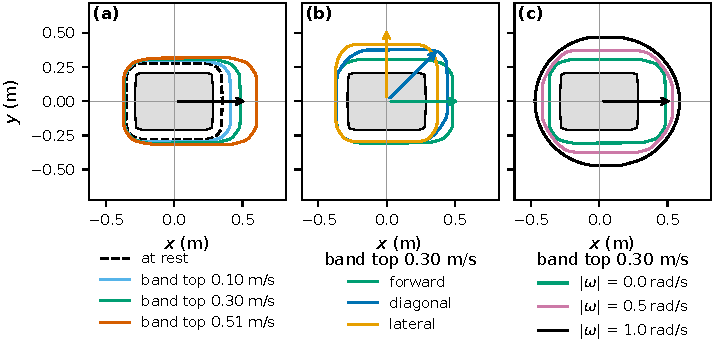
\includegraphics[width=\textwidth]{figures/fig2_field_geometry.pdf}
\caption{Protective-field geometry from Equations~(\ref{eq:field})--(\ref{eq:extent}) on the measured footprint. (\textbf{a}) The at-rest field and the three band fields for straight forward travel without rotation. (\textbf{b}) The band-1 field for travel in three directions: forward, diagonal and lateral. (\textbf{c}) The band-1 field for forward travel at three yaw rates, showing the rotation sweep and coupling terms. Generated by \texttt{paper/figures/scripts/fig2\_field\_geometry.py} from \texttt{pfbnav/safety/pfb\_field.py} and the configuration.\label{fig:fields}}
\end{figure}

\textbf{The field in force.} The layer never sizes the field below true motion. Its composed speed is $s = \max(\|\hat{\mathbf{v}}_{xy}\|, \|\mathbf{u}^{\text{app}}_{xy}\|)$, the larger of the estimated speed and the speed of the command the base is executing after the limiter, and its yaw rate is whichever of $\hat{\omega}$ and $\omega^{\text{app}}$ has the larger magnitude: the command alone understates motion while decelerating, and the lagged estimate understates it while accelerating. The field faces the direction of the dominating signal. A standstill detector with hysteresis classifies the robot as at rest: a resting robot is moving once $s > s_{\text{out}} = 0.02$\,m/s or $|\omega| > \omega_{\text{out}} = 0.0592$\,rad/s, and a moving robot is at rest once $s \le s_{\text{in}} = 0.01$\,m/s and $|\omega| \le \omega_{\text{in}} = 0.0296$\,rad/s. The rotational thresholds are the translational ones divided by $\rho_{\text{out}}$, so no body point at rest moves faster than the translational threshold. The field in force is $h_{\text{rest}}$ at rest and $h_{V_{\ell(s)}}$ otherwise.

\textbf{Breach, latch and restart.} A valid sector inside the field in force ($\chi_k = 1$ and $r_k < \rho(\psi_k)$), or any invalid sector, is a breach. A breach while no stop is pending \emph{triggers} a protective stop; the stop becomes active $t_r$ later, and from then on the layer replaces every command by zero. An active stop is latched: it holds while the field is breached and for a restart delay of $t_d = 2.0$\,s after the field last came clear. Release then requires the restart condition: the \emph{whole} field that the commanded twist would select must be clear, where a twist at or below both standstill exit thresholds keeps the at-rest field and anything faster selects the band of its reachable speed along its translation, with its own rotation sweep. Two approach rules follow the whole-field test: the commanded translation has no component toward any breaching point, and the velocity of the footprint point closest to each breaching point has no component toward it. A stopped robot may therefore be approached to the minimum margin, but may never drive toward an intrusion. The creep regime, slow enough to keep the at-rest field, is the way out of the thin shell that containment and nesting leave around a stopped robot; for classical baselines it is scripted by a declared recovery behaviour (Section~\ref{sec:comparators}), and for learned policies it is a learnable skill, since the stop flag is part of the observation.

\textbf{The receding release.} A stop triggered while creeping ends a few millimetres closer to its cause, inside the at-rest field, which no twist can then clear. A robot held at rest with its at-rest field breached is therefore released, after $t_d$, for a creep twist under which every point inside the at-rest field strictly recedes from the footprint, by both approach rules applied strictly and for every footprint point within the field's thickness of the point. Those points are exempt from re-triggering only while the command keeps receding at creep speed; any other breach triggers normally, and invalid sectors still block. Its industrial counterpart is an operator reset followed by a reduced-speed manoeuvring mode; this release is automatic, and therefore less conservative than hardware (Appendix~\ref{app:realism}).

\textbf{Warning field.} Each band also carries a warning field, larger than the protective field (depth $1.5\,D(V)$ plus 0.05\,m ahead, 0.02\,m abeam, behind and at rest). Its entries are counted as a secondary near-miss metric; it never acts on the command and is not part of the observation.

\subsection{Navigation Stack}\label{sec:navstack}

\textbf{Map baking.} Each layout is rasterised into a planner grid of 0.05\,m cells. Obstacles that are absent from the map by design (Section~\ref{sec:design}) are excluded from it, so the planner never knows them while the scanners and the safety layers see them.

\textbf{Two-tier inflation and A*.} The global plan is deliberately not footprint-complete. Cells within the lethal radius of an obstacle, the inscribed half-width plus a 0.10\,m margin ($0.3086$\,m), can never hold the robot's centre at any heading and are not entered. A soft cost falls linearly from 1 at the lethal radius to 0 at the circumscribed radius plus 0.03\,m ($0.3674$\,m) and discourages, without forbidding, the band in between: a move into a cell of soft cost $c$ costs its length times $(1 + \kappa_s c)$, with weight $\kappa_s = 1$. An 8-connected A* search with the octile heuristic, which is admissible, finds the cheapest grid path, and line-of-sight simplification removes waypoints whose replacing segment stays clear of lethal cells, tested over every cell the segment touches. A failed search is a named status, never a substitute path. The lethal and soft margins were set by a declared criterion on the routes' traversability under a free-orientation oracle (Section~\ref{sec:design}).

\textbf{Route tracking.} Progress is the arc length $s$ of the robot's projection onto the route. The projection is monotonic, searched within 1.0\,m of arc ahead of the previous one, so that a route doubling back on itself cannot make the tracker jump. The tracked waypoint lies 0.8\,m of arc ahead; it and the goal are given to the controller as distance and bearing in the body frame.

\subsection{Definitions}\label{sec:definitions}

The evaluation rests on four definitions.

\begin{Definition}[Protective stop]\label{def:stop}
A protective stop is a trigger event of the certified layer: a step at which the field in force is breached while no stop is triggered or latched. A breach that persists, and the latched stop that follows it, are counted once, at the trigger.
\end{Definition}
% source: pfbnav/safety/certified.py::CertifiedLayer.step ("triggered"); pfbnav/envs/step_loop.py::StepLoop._count

\begin{Definition}[Scan-fault stop]\label{def:scanfault}
A scan-fault stop is a protective stop decided on a packet that failed the plausibility check through every re-render and was replaced by the fail-safe (Section~\ref{sec:sensing}). Scan-fault stops are excluded from the primary stop count and reported beside it.
\end{Definition}
% source: pfbnav/envs/step_loop.py::LoopCounters.scan_fault_stops; preregistration/endpoints.yaml H1.scan_faults (A25)

\begin{Definition}[Ground-truth contact]\label{def:contact}
Contact is decided by the simulator's collision check and by nothing else: the chassis (with the scanner housings) against every object outside the robot, including the floor, so that a tip-over counts, and the wheels against the same set without the floor. An episode in which contact occurs ends as a collision. Range readings never define a collision.
\end{Definition}
% source: pfbnav/sim/contact.py::RobotContact; CLAUDE.md hard rule 4

\begin{Definition}[Unrecoverable stop]\label{def:unrecoverable}
An episode that reaches its step horizon while a protective stop is latched and the robot cannot legally move again, either because the restart condition blocks every release or because the robot is at rest with its own field breached, ends as an unrecoverable stop. It is distinguished from a timeout, in which the robot was free to move.
\end{Definition}
% source: pfbnav/envs/reward.py::episode_outcome

\noindent The primary metric is the number of protective stops per 100\,m driven, pooled over episodes as total stops (excluding scan-fault stops) divided by total distance:
\begin{equation}
\text{SP100} = 100\,\frac{\sum_e \big(N^{\text{stop}}_e - N^{\text{fault}}_e\big)}{\sum_e d_e}.
\label{eq:sp100}
\end{equation}
% source: pfbnav/envs/step_loop.py::LoopCounters.stops_per_100m; pfbnav/eval/runner.py (pooled, not averaged)
The problem addressed is to filter the controller's command so that the certified layer triggers as rarely as possible, without giving up the task: reaching the goal within the horizon and without contact.

%%%%%%%%%%%%%%%%%%%%%%%%%%%%%%%%%%%%%%%%%%
\section{The Protective-Field Barrier}\label{sec:pfb}

The PFB is a safety filter between the controller and the certified layer. Its safe set is the complement of the certified safety function's own trigger set: every valid scan return must remain outside the protective field of the regime in which the robot will be. It reads the same scan, the same velocity estimate and the same applied command as the certified layer, and builds its field from the same configuration keys, but it is implemented independently of the emulator and the two are cross-checked only in tests. Throughout, $\mathbf{u} = (v_x, v_y, \omega)$ is a candidate command, $\mathbf{u}^{\text{nom}}$ the controller's command and $\mathbf{u}^{-}$ the command the base applied at the previous step.

\subsection{Regimes and the Per-Sector Barrier}\label{sec:barrier}

The certified layer is in one of four regimes $\lambda \in \Lambda = \{\text{rest}, 0, 1, 2\}$: at rest, or moving in one of the three speed bands. Because the band is chosen from the reachable speed and switches discretely, the PFB solves one problem per regime and keeps the best feasible answer (Section~\ref{sec:qp}); this banded form, PFB-(b), is the one adopted. A continuous variant, PFB-(a), which sizes the field from the reachable speed itself, is evaluated only as an exploratory ablation (Section~\ref{sec:hypotheses}). \todo{confirm against implementation: PFB-(a)'s QP is not implemented yet.}

For regime $\lambda$, let $\rho_\lambda(\psi;\theta,W)$ be the field's boundary distance (Equation~(\ref{eq:extent})) for travel direction $\theta$ and yaw rate $W$, built from $h_{\text{rest}}$ (Equation~(\ref{eq:restfield})) for $\lambda = \text{rest}$ and from $h_{V_\lambda}$ (Equation~(\ref{eq:field})) for a band. The barrier of a valid sector $k$, with return point $\mathbf{p}_k = r_k(\cos\psi_k, \sin\psi_k)$, is
\begin{equation}
h^\lambda_k = r_k - \rho_\lambda\big(\psi_k;\ \theta_0,\ W_0\big) - \delta,
\label{eq:barrier}
\end{equation}
% source: pfbnav/safety/pfb.py::PFB._now
evaluated at the present motion: $\theta_0$ is the heading of $\mathbf{u}^{-}$ if its speed exceeds the estimated speed and of $\hat{\mathbf{v}}$ otherwise, and $W_0 = \max(|\hat\omega|, |\omega^{-}|)$. The binning penalty $\delta = 0.5$\,mm is the measured scan residual against a wall face at the upper bound of its bracket ($-0.27$ to $+0.50$\,mm). $h^\lambda_k \ge 0$ for every valid sector means that regime $\lambda$'s field is clear.

\subsection{Prediction and the Discrete-Time Barrier Condition}\label{sec:cbf}

A candidate command moves each return relative to the body. Over the prediction horizon $\tau = \Delta t + \tau_{\text{lag}}$, one control step plus a declared lag allowance $\tau_{\text{lag}} = 0.05$\,s, the return is predicted at
\begin{equation}
\mathbf{p}'_k(\mathbf{u}) = \mathbf{R}(-\omega\tau)\big(\mathbf{p}_k - \tau\,(v_x, v_y)\big),
\label{eq:prediction}
\end{equation}
% source: pfbnav/safety/pfb.py::PFB._rows
and, with $\mathbf{p}'_k(\mathbf{u})$ from Equation~(\ref{eq:prediction}), the predicted barrier is
\begin{equation}
g^\lambda_k(\mathbf{u}) = \|\mathbf{p}'_k(\mathbf{u})\| - \rho_\lambda\big(\angle\mathbf{p}'_k(\mathbf{u});\ \theta(\mathbf{u}),\ W(\mathbf{u})\big) - \delta,
\label{eq:predicted}
\end{equation}
% source: pfbnav/safety/pfb.py::PFB._rows
where the field faces the candidate's own direction of travel when its speed is at least the estimated speed, $\theta(\mathbf{u}) = \operatorname{atan2}(v_y, v_x)$, and the estimate's direction otherwise, and $W(\mathbf{u}) = \max(|\hat\omega|, |\omega|)$: as in the certified layer, the field is never sized below the larger of the estimated and the commanded motion. The filter admits $\mathbf{u}$ in regime $\lambda$ only if, for every valid sector,
\begin{equation}
g^\lambda_k(\mathbf{u}) \;\ge\; (1 - \alpha\,\Delta t)\,\big[h^\lambda_k\big]^+ ,
\label{eq:cbf}
\end{equation}
% source: pfbnav/safety/pfb.py::PFB.filter (rhs = (1 - alpha dt) max(h_now, 0))
with class-$\mathcal{K}$ gain $\alpha$. This is a deliberate departure from the standard discrete-time barrier condition $g \ge (1-\alpha\Delta t)h$. Within one regime's field the clearance may decay at most at rate $\alpha$, as usual. Across regimes, however, the barrier of a field the robot is not yet in may already be negative, and the standard form would then permit entering it, provided the violation shrinks. Entering a breached field is itself the event to be avoided, since the certified layer acts at once; the clipped right-hand side requires a regime whose field is breached now to be clear after one step, which in practice rules it out. The gain $\alpha$ is provisional at 2.0\,s$^{-1}$ and is tuned under a pre-declared rule (Section~\ref{sec:comparators}). \todo{Final value of $\alpha$ after tuning.}

\subsection{The Quadratic Program}\label{sec:qp}

For each admissible regime, the filter seeks the admissible command closest to the nominal one,
\begin{equation}
\begin{aligned}
\min_{\mathbf{u}}\quad & (\mathbf{u} - \mathbf{u}^{\text{nom}})^\top \mathbf{W}\, (\mathbf{u} - \mathbf{u}^{\text{nom}}), \qquad \mathbf{W} = \operatorname{diag}(1,\, 1,\, \rho_{\text{out}}^2),\\
\text{s.t.}\quad & \text{Equation~(\ref{eq:cbf}) for every valid sector},\\
& |v_x| + |v_y| + L|\omega| \le 0.95\, v_{\text{rim}}, \quad |v_x| \le v_{x,\max},\ |v_y| \le v_{y,\max},\ |\omega| \le \omega_{\max},\\
& \text{the limiter's one-step envelope (Equation~(\ref{eq:limiter})) about } \mathbf{u}^{-},\\
& \|(v_x, v_y)\| \le \bar{V}_\lambda, \qquad |\omega| \le 0.9\,\omega_{\text{out}} \ \text{ if } \lambda = \text{rest}.
\end{aligned}
\label{eq:qp}
\end{equation}
% source: pfbnav/safety/pfb.py::PFB._static (constraints), PFB._solve (cost), PFBConfig.weight_yaw
The weight on the yaw rate makes one rad/s of turning cost what the footprint's outermost point moves, $\rho_{\text{out}} = 0.3374$\,m. The wheel-speed constraint is the polytope~(\ref{eq:budget}), eight half-spaces, at the filter's share. The speed limit $\bar{V}_\lambda$ keeps the robot in its regime under reach: $V_\lambda - a_{\max}T$ for bands 0 and 1, less a margin of 0.002\,m/s, so that an estimate slightly above the command cannot tip the certified layer into the next band; $v_{\text{cap}}$ for the top band; and, at rest, the creep speed $0.9\,s_{\text{out}} = 0.018$\,m/s, with the yaw rate held to $0.9\,\omega_{\text{out}}$, so that a creeping robot keeps the at-rest field. The limiter's envelope is non-convex as a whole, since it depends on whether the command reduces speed, and is imposed as two convex cases solved in turn: holding or accelerating, $\|(v_x,v_y) - (v^-_x,v^-_y)\| \le a_{\max}\Delta t$; and, if that case has no solution, braking, $\|(v_x,v_y)\| \le \|(v^-_x,v^-_y)\|$ and $\|(v_x,v_y) - (v^-_x,v^-_y)\| \le a_{\text{dec}}\Delta t$; in both, $|\omega - \omega^-| \le \alpha_{\max}\Delta t$. The discs are imposed as inscribed 16-sided polygons, so every point of the feasible set is reachable.

\textbf{Admissible regimes.} The rest regime is admissible only while a mirror of the certified layer's standstill detector, with the same hysteresis, classifies the robot as at rest; a band is admissible only if it is not below the band that the estimated speed selects, because the estimate lags and the certified layer composes it with the command. If the nominal command satisfies every constraint and every barrier row of some admissible regime, it passes unchanged. Otherwise each admissible regime is solved, and the feasible solution of least cost is applied.

\textbf{Linearise, check, fall back.} The barrier rows of Problem~(\ref{eq:qp}) are non-convex in $\mathbf{u}$ and are linearised. Each regime's problem is linearised about a reachable point near the nominal command: the nominal step from $\mathbf{u}^-$ clipped to the envelope, then to the regime's speed limit and the yaw box, then scaled into the wheel polytope. In translation each row keeps its tangent; in the yaw rate, where the field grows convexly with $|\omega|$ and has a kink at $|\omega| = |\hat\omega|$, each row is replaced by its two chords over a trust interval of $\pm 0.05$\,rad/s about the linearisation point, which lie below the true row and describe it conservatively and convexly. The linearised rows are tightened by 0.5\,mm, and rows whose linearised slack exceeds 0.5\,m are omitted from the QP\@. Each QP is solved by an interior-point method (Clarabel~\citep{goulart2024clarabel}). Its solution is accepted only if it satisfies every \emph{true} row~(\ref{eq:cbf}), with no tolerance, and every constraint; otherwise the problem is linearised once more, about that solution, or about the braking command below if the first problem was infeasible, and solved again. If no regime yields an accepted solution, the filter applies maximum braking within the limiter,
\begin{equation}
(v_x, v_y) \leftarrow (v^-_x, v^-_y)\Big[1 - \frac{a_{\text{dec}}\Delta t}{\|(v^-_x, v^-_y)\|}\Big]^+,\qquad
\omega \leftarrow \operatorname{sgn}(\omega^-)\,\big[|\omega^-| - \alpha_{\max}\Delta t\big]^+.
\label{eq:fallback}
\end{equation}
% source: pfbnav/safety/pfb.py::PFB.fallback
Before the step is declared infeasible, this braking command~(\ref{eq:fallback}) is itself checked against the true rows of every admissible regime; if it satisfies them, the step is recorded as a feasible braking step, because the 0.5\,mm tightening can exceed the decay that~(\ref{eq:cbf}) allows close to a field boundary and hide that holding still is safe. Otherwise the step is flagged infeasible and counted; the infeasibility count is reported per method and stratum. Any invalid sector in the scan also triggers the fallback, flagged as unobserved: the filter does not plan through space it has not observed. Figure~\ref{fig:pfbstep} illustrates one filter step.

\begin{figure}[H]
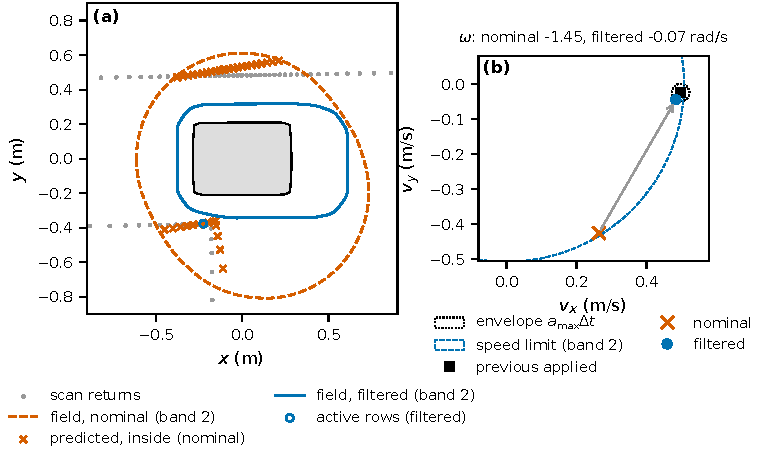
\includegraphics[width=\textwidth]{figures/fig5_pfb_step.pdf}
\caption{One PFB step on a tuning route: the step at which the filter changed the nominal command most. (\textbf{a}) Body frame: the scan returns and the footprint; the field the nominal command would select (dashed), with the returns predicted one horizon ahead under that command marked where they fall inside it; and the field of the filtered command's regime (solid), with its active barrier rows (least slack) circled. (\textbf{b}) The plane of translation: the previous applied command, the nominal and filtered commands, the limiter's envelope about the previous command and the speed limit of the filtered command's regime; the yaw rates are given above the panel. The nominal command here is the scan-blind ideal route tracker of the acceptance step, because no learned policy has been trained yet. \todo{Replace the nominal command with a learned (L5) command after training.} Generated by \texttt{paper/figures/scripts/fig5\_pfb\_step.py} from the emulator and \texttt{pfbnav/safety/pfb.py}.\label{fig:pfbstep}}
\end{figure}

\textbf{Behaviour under the latch.} While the certified layer holds a protective stop, the filter passes only commands that the restart condition could release, and replaces every other command by zero. A command is releasable if it is a creep (at or below both standstill exit thresholds) whose at-rest field is clear or under which every point inside that field strictly recedes, or a faster twist whose own band field, along its translation and swept for its yaw rate, is clear. The recovery behaviour's creep commands therefore pass unaltered when releasable.

\textbf{Design parameters.} The trust interval (0.05\,rad/s) and the band speed margin (0.002\,m/s) were selected on tune routes to remove failures observed in closed loop, and are design parameters rather than measurements. Their sensitivity, at $\pm 50\,\%$, is reported after $\alpha$ is tuned. \todo{Sensitivity results.} The filter was verified, before any training, by an acceptance step in which a scan-blind ideal route tracker drove the 60 tune routes through the PFB with the certified layer beneath, and every certified stop had to be attributed to a named cause: prediction error, an unobserved sector, infeasibility or creep. On the final code, the decisive simulator run reached the goal on 48 of the 60 routes (12 stalled on unmapped obstacles) with five certified stops, all attributed (four infeasible, one prediction error in a tight turn), and no contact, including in braking rollouts from every fallback step. The emulator run, with the sector scan, agreed: 48 goals, 29 stops, all attributed, no contact. Part of the filter's cost is conservatism: evaluating the barrier rows over the realised motion fraction, with the 0.5\,mm tightening, raised the emulator's fallback steps from 243 to 317 (+30\,\%) against the earlier formulation, with the same goals and stalls.

\subsection{Learning Design}\label{sec:learning}

\textbf{Observation.} The policy observes an 82-dimensional vector (Table~\ref{tab:observation}). It is pose-agnostic, with no absolute position or heading, so a policy cannot memorise a layout instead of reacting to what it senses, and validity is a separate channel, so that ``unobserved'' and ``obstacle at that range'' are never the same input. The stop flag tells the policy that a protective stop is latched; creep departure from a stop is therefore learnable.

\begin{table}[H]
\caption{The 82-dimensional observation. Ranges are those of the 36-sector policy stream; velocities are the estimated body velocity; the lookahead point lies 0.8\,m of arc ahead on the route.\label{tab:observation}}
\newcolumntype{L}{>{\raggedright\arraybackslash}X}
\begin{tabularx}{\textwidth}{lcL}
\toprule
\textbf{Block} & \textbf{Channels} & \textbf{Content and scaling}\\
\midrule
Scan & 36 & range / 5.0\,m, in $[0,1]$\\
Validity & 36 & 1 where the sector is observed, 0 where it is not\\
Velocity & 3 & $(\hat v_x/0.5,\ \hat v_y/0.5,\ \hat\omega/1.5)$, clipped\\
Lookahead & 3 & $(d_{\text{wp}}/0.8,\ \sin\beta_{\text{wp}},\ \cos\beta_{\text{wp}})$\\
Goal & 3 & $(\min(d_g/18, 1),\ \sin\beta_g,\ \cos\beta_g)$\\
Stop flag & 1 & 1 while a protective stop is active, else 0\\
\midrule
Total & 82 & \\
\bottomrule
\end{tabularx}
\end{table}
% source: pfbnav/envs/observation.py (BLOCKS); configs/base.yaml env.observation.goal_scale, planner.lookahead

\textbf{Action.} The action $\mathbf{a} \in [-1,1]^3$ is scaled by each axis's own ceiling, $\mathbf{u}^{\text{req}} = \mathbf{a} \odot (0.5,\ 0.5,\ 1.5)$, so a normalised magnitude never asks for more on one axis than another's envelope allows. The request then passes through the PFB (for the filtered methods), the certified layer and the base's limits (Figure~\ref{fig:architecture}).

\textbf{Reward.} The per-step reward is
\begin{equation}
r = k_p\,\Delta s - c_t - k_{\text{stop}}\,\mathbb{1}[\text{stop triggered}] - k_{\text{int}}\,I - k_{\text{prox}}\,P + r_{\text{goal}}\,\mathbb{1}[\text{goal}] - r_{\text{contact}}\,\mathbb{1}[\text{contact}],
\label{eq:reward}
\end{equation}
% source: pfbnav/envs/reward.py::step_reward; configs/base.yaml reward
with progress weight $k_p = 5.0$ on the arc length $\Delta s$ gained along the route, time cost $c_t = 0.01$ per step, stop penalty $k_{\text{stop}} = 5.0$ charged once on each trigger, goal bonus $r_{\text{goal}} = 200$ and contact penalty $r_{\text{contact}} = 200$. Charging the stop on its trigger, rather than on every stopped step, avoids paying the policy to break a latch it cannot break. The intervention term is the PFB's alone,
\begin{equation}
I = \Big\|\big(\mathbf{u}^{\text{req}} - \mathbf{u}^{\text{PFB}}\big) \oslash (0.5,\ 0.5,\ 1.5)\Big\|^2,\qquad I = 0 \text{ without the filter},
\label{eq:intervention}
\end{equation}
% source: pfbnav/envs/reward.py::intervention_cost (ruled 2026-10-24)
with $k_{\text{int}} = 0.1$, where $\mathbf{u}^{\text{PFB}}$ is the filter's output before the certified layer and the base's limits; certified overrides are excluded, so that the term never acts as a hidden stop penalty. \todo{My decision: under the latch the filter zeroes non-releasable commands, so the term charges a policy that keeps requesting motion during a stop; confirm whether latched steps should count.} The proximity cost $P = \operatorname{clip}\big((0.5 - r_{\min})/0.5,\ 0,\ 1\big)$, with $r_{\min}$ the nearest valid filter-stream range from the body origin, is weighted by $k_{\text{prox}} = 0$ for the proposed method and $k_{\text{prox}} = 2.0$ for the shaped variant L1. \todo{confirm against implementation: L4's configuration does not exist yet; its $k_{\text{prox}}$ to be stated.}

\textbf{Termination.} An episode ends with success when the robot is within 0.25\,m of the goal, and with a collision on any ground-truth contact (contact takes precedence on the same step). It is truncated after 4{,}000 steps (200\,s), as a timeout or as an unrecoverable stop (Definition~\ref{def:unrecoverable}).

\textbf{SAC with the filter in the loop.} The proposed method, L5, trains Soft Actor-Critic~\citep{haarnoja2018sac} with the PFB inside the environment's step, so that every transition the agent learns from was filtered, and keeps the filter at deployment. The configured hyperparameters are a learning rate of $3\times 10^{-4}$, a replay buffer of 200{,}000 transitions, 2{,}000 steps before learning starts, batches of 256, target smoothing $0.005$, discount $0.99$, one gradient update per environment step, the learned entropy temperature, and two hidden layers of 256 units for actor and critics. The training budget is 300{,}000 steps, to be fixed after the compute gate G2. \todo{confirm against implementation: no filtered policy has been trained yet; confirm how the stored action relates to the filtered command, and the final training budget after G2.} Training uses a declared sensor-dropout augmentation on the policy stream only, never on the filter stream: with probability 0.10 an episode begins with a contiguous arc of 1 to 6 policy sectors blinded for the whole episode, and every sector drops out independently with probability 0.01 per step; a dropped sector reads range 0 and is flagged invalid. Training scenarios are drawn in equal thirds from the three clearance strata (667 per stratum) at an unmapped-obstacle rate of 0.25, each training seed visiting the whole set in its own permutation, shared by every method's seed of the same index, without a curriculum.

%%%%%%%%%%%%%%%%%%%%%%%%%%%%%%%%%%%%%%%%%%
\section{Experimental Design}\label{sec:design}

The hypotheses, comparators, endpoints, gates and scenario-set construction were fixed in a preregistration before any method was trained, and every later change was made by a dated amendment recorded before its effect was known. This section transcribes the preregistered design; where the preregistration has yet to fix an element, the text says so.

\subsection{Layouts, Scenarios and Splits}\label{sec:layouts}

\textbf{Warehouse layouts.} Each scenario is a procedurally generated warehouse hall of $14 \times 10$\,m with 0.2\,m perimeter walls and two to four rows of shelving 0.8\,m deep and 1.6\,m tall, well above the scan plane, so shelves are sensed at scanner height. Row lengths are 0.70--0.92 of the usable span, rows alternate which end they leave open, and 1.2\,m is kept clear at each row end so the robot can turn out. Start and goal are drawn so that at least 1.5\,m of the planned route lies between two shelf rows; otherwise the layout's clearance stratum need not describe the episode. Figure~\ref{fig:layout} shows an example.

\textbf{Clearance strata.} Aisles are stratified by per-side clearance, the gap on each side of a centred, aligned robot, rather than by aisle width: narrow $[0.1987, 0.2687]$\,m, medium $[0.2687, 0.40]$\,m and wide $[0.40, 0.80]$\,m. The narrow floor follows a declared rule: the smallest clearance at which three gaps to the aisle walls are non-negative as the layer evaluates them on the 120-sector scan, namely the at-rest field of a centred robot, the at-rest field of a robot displaced by the committed tracking bound of 0.05\,m, and the moving field at that offset in every band a reachable speed selects (0.1687\,m under the field of Section~\ref{sec:emulator}), plus a deliberate buffer of 0.03\,m.

\textbf{Route validity.} Every built route must be traversable by a free-orientation oracle that chooses the robot's heading freely along the route: band 0's field must be clear at the start along the initial direction, clear on arrival at the goal, and clear in between, including the rotation sweep of tangent tracking at bends. On failure the goal is re-drawn, never the layout, and rejections are logged by cause and stratum. The planner's lethal and soft margins (Section~\ref{sec:navstack}) were set by the same oracle criterion.

\textbf{Splits and identity.} Layouts are identified by their seed, their geometry's hash and the generator's code hash, and are regenerated and verified at load. Seeds are drawn from disjoint ranges: training $[1, 2)\times 10^6$, tuning $[2, 3)\times 10^6$, test $[3, 4)\times 10^6$, and a pilot range $[9, 10)\times 10^6$ for development, from which nothing may appear in a reported result. Test layouts are locked and are never used for tuning, debugging, reward design or plots during development. The tuning set has 20 scenarios per stratum at the training obstacle rate (Section~\ref{sec:unmapped}); a second, disposable tuning set of 20 per stratum at rate 1.0 measures the seed variability and stop rates on which the analysis plan depends; the pilot set has 150 distinct narrow-stratum scenarios. \todo{Test-set size: amendment A14, fixed after the compute gate G2 and the power analysis; not yet preregistered.}

\begin{figure}[H]
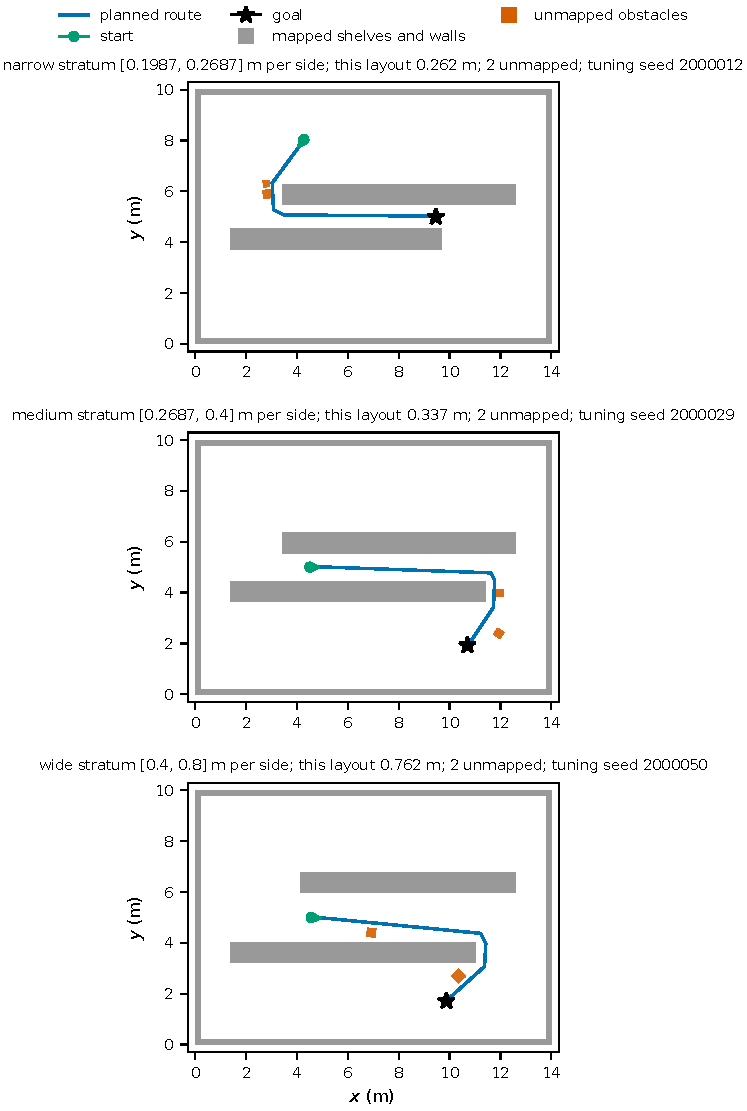
\includegraphics[width=\textwidth]{figures/fig4_layout.pdf}
\caption{An example generated layout from the tuning set (never the test set), with the planned route, the shelf rows and their per-side clearance stratum, and the unmapped obstacles placed near the route, which the planner does not know. Generated by \texttt{paper/figures/scripts/fig4\_layout.py} from the scenario's recorded seed through the project's generator, baking and planner.\label{fig:layout}}
\end{figure}

\subsection{Obstacles Absent from the Map}\label{sec:unmapped}

The central condition of the study is a world that differs from the map. Unmapped obstacles are square, 0.25--0.60\,m on a side and 0.80\,m tall (above the scan plane, so they are sensed though not mapped), one or two per episode when an episode has any, and are excluded from the planner's map. The rate of episodes with unmapped obstacles is 0.25 in training and tuning; the test set has a \emph{mapped-only} condition (rate 0) and an \emph{unmapped-static} condition (rate 1.0). The rate is a shared environment parameter, identical for every learned method.

\textbf{Route-relative placement.} Obstacles are placed relative to the planned route, in every split. The offset from the route to the obstacle's nearest surface is uniform on $[0, 0.6]$\,m, except for the first obstacle, whose offset is uniform on $[0, 0.3]$\,m, so every scenario has a surface within 0.3\,m of the route; side is uniform, and position is uniform over the route's arc length excluding the first 2\,m and the last 1\,m. Each obstacle keeps 0.15\,m from any shelf or wall, so it never merges into geometry the planner already knows.

\textbf{Bypass rule.} An obstacle is kept only if, judged jointly with every unmapped obstacle already placed, the robot can get from start to goal keeping its centre at least the half-width plus the narrow floor ($0.2086 + 0.1987 = 0.4073$\,m) from every surface and never further than $W = 1.0$\,m from the planned route. A stack that never replans cannot use a detour through another aisle, so the gap past an obstacle must itself be passable within the route's corridor. A rejected obstacle is re-sampled, never the layout. In the unmapped-static test sets at least 90\,\% of scenarios must have an obstacle surface within 0.3\,m of the route.

\subsection{Comparators}\label{sec:comparators}

Table~\ref{tab:comparators} lists the methods. Every method runs above the same certified layer, on the same planned route, with the same scan streams and actuation limits.

\begin{table}[H]
\caption{Comparators and their roles. B: classical baselines; L: learned methods; A1 and L5-nowp: exploratory arms. Retired identifiers (B4, B5) are not reused.\label{tab:comparators}}
\begin{adjustwidth}{-\extralength}{0cm}
\newcolumntype{L}{>{\raggedright\arraybackslash}X}
\begin{tabularx}{\fulllength}{lLcl}
\toprule
\textbf{ID} & \textbf{Method} & \textbf{PFB} & \textbf{Role}\\
\midrule
B1 & Holonomic Pure Pursuit along the route; the industrial status quo, relying on the safety scanners to stop it & no & H1, H1N\\
B2 & Regulated Pure Pursuit: slows on curvature and near obstacles & no & H1, H1N\\
B3 & Holonomic dynamic window over $(v_x, v_y, \omega)$~\citep{fox1997dwa} & no & H1, H1N\\
B6 & Holonomic MPPI with a cost on the certified layer's own band fields (not the PFB's) & no & H1, H1N\\
B7 & B2's tuned parameters plus the PFB, no learning & yes & H5, H3\\
L1 & SAC with proximity shaping, no filter & no & H1, H1N\\
L2 & SAC-Lagrangian: expected protective stops per episode constrained, unshaped reward & no & H1, H1N\\
L3 & A policy trained without the filter, wrapped by it after training (post-hoc filtering) & yes & H1, H1N\\
L4 & SAC trained with the PFB in the loop, with proximity shaping & yes & H2\\
L5 & SAC trained with the PFB in the loop, without proximity shaping (proposed) & yes & H1, H2, H1N, H5\\
A1 & Unicycle ablation of L5 & yes & H4\\
L5-nowp & L5 without the planner: lookahead channels removed, straight-line progress reward & yes & exploratory\\
\bottomrule
\end{tabularx}
\end{adjustwidth}
\end{table}
% source: configs/methods.yaml; preregistration/endpoints.yaml (A16); AMENDMENTS.md A16, A23; docs/decision_log.md 2026-10-03 (L2), 2026-10-24 (B7)

\textbf{The classical set.} B1, B2, B3, B6 and B7 share a declared recovery behaviour and a declared route cap, and an equal tuning budget on the tuning set only: each of B1, B2, B3 and B6 is tuned by a seeded random search of 24 candidates over declared ranges, the first being its initial values, and the candidate selected is the one with the fewest protective stops per 100\,m among those within five percentage points of the best success rate, ties broken by mission time; a winner on a range boundary is reported, never extended. B7 reuses B2's tuned parameters and is tuned only in $\alpha$. The learned arms share one set of SAC hyperparameters rather than a tuning budget each. The recovery acts when a stop's restart stays blocked for 1.0\,s beyond the restart delay: it creeps at 0.018\,m/s, translation only, in the best of 72 candidate directions judged by the field each would select, for at most 0.30\,m per attempt and at most five attempts per episode. The route cap is the fastest band whose field is clear of the \emph{mapped} obstacles at each point of the route, with a yaw-rate cap at bends, anticipated over 0.10\,m and limited to a deceleration of 0.5\,m/s$^2$; it is computed offline from the map, controllers may go slower but never faster, and learned methods receive neither cap nor recovery. B6 is the decisive comparator for H1: a hand-designed controller that avoids what stops it.

\textbf{Learned methods.} L1, L4 and L5 share the SAC configuration of Section~\ref{sec:learning}. L2 constrains the expected number of protective stops per episode to at most $d$, enforced by a Lagrange multiplier with dual ascent and a separate cost critic, with the unshaped task reward and no stop penalty; $d$ is chosen from $\{0.05, 0.1, 0.2\}$ on the tuning set, and the method is validated first on a toy problem where the constraint is known to bind. L3 is a separate, labelled baseline: wrapping a policy trained without the filter is not the proposed method.

\textbf{Tuning the filter gain.} The PFB's gain $\alpha$ is tuned once, with B7, over $\{1, 2, 5, 10, 20\}$\,s$^{-1}$ on the tuning set at the training obstacle rate, and then frozen for L3, L4, L5 and B7. Among the settings whose success rate is within 5 percentage points of the best, the one with the fewest protective stops per 100\,m is selected, ties broken by mission time. \todo{The grid and the selection rule are to be declared in the preregistration before tuning (ruled 2026-10-24); not yet amended.}

\textbf{Oracle reference.} A privileged oracle tracker follows the mapped route at the speed and body yaw of the free-orientation oracle's schedule, computed over every obstacle, mapped and unmapped. It is never a comparator; it is the positive control of the learned-method gate and its mission time is reported as a reference line.

\subsection{Seeds, Gates and Horizon}\label{sec:seeds}

\textbf{Gates.} Four pre-declared gates protect the evaluation.
\begin{itemize}
\item \textbf{G0, contact validation.} Six positive cases (front wall head-on, side wall lateral, scanner-housing corner, wheel edge, rear wall, and a raised obstacle meeting a scanner housing) approached at 0.1\,m/s must be detected within one step of the geometric prediction, and a parallel pass with a 10\,mm gap must produce no false contact, both in the gate script and inside the environment's step loop.
\item \textbf{G1b, closed-loop tracking.} Forward, lateral, diagonal and translate-while-rotating profiles of 5\,m at 0.10--0.50\,m/s, three repetitions, must stay within 0.05\,m peak and 0.02\,m RMS cross-track error and 5$^\circ$ final heading error; the velocity ceilings are the gate's output.
\item \textbf{G2, compute budget.} At least 25 steps/s aggregated over parallel instances on the training host, essentially no steps over the per-step budget, and runs with more than 0.1\,\% scan-faulted steps flagged.
\item \textbf{G4, learned-method pilot.} Each learned method's pilot seed (from the pilot range, never entering H1 or H2) must pass integrity checks, a learning criterion (success at least 0.20 over the last 10\,\% of training episodes and at least 0.15 above the first 10\,\%) and a checkpoint criterion on the 60 tuning scenarios (success at least 0.30, at most 0.10 of episodes with contact). Its controls must behave as declared before any verdict is read: zero action must fail with all timeouts, and the privileged oracle tracker must pass.
\end{itemize}
After G4 passes, every confirmatory seed trains unconditionally and stays in the analysis whatever its outcome; no seed is rerun, replaced or dropped. \todo{Seed count per learned method: the preregistration states five seeds averaged per scenario; later rulings set the count by the power analysis (capped at 20, subject to G2) pending amendment A14. Reported as an inconsistency; not resolved here.}

\textbf{Horizon.} An episode lasts at most 4{,}000 steps (200\,s). The horizon is derived, not chosen: it must cover the privileged oracle schedule of every traversable built route with a margin of 1.3, which is checked over every built set.

\subsection{Metrics}\label{sec:metrics}

The primary endpoint is protective stops per 100\,m, Equation~(\ref{eq:sp100}), with scan-fault stops excluded and reported beside it per method; scan faults are reported prominently if they differ materially between methods. Success rate and mission time are reported beside the stop rate for every comparison, in the same table. Secondary quantities are the unrecoverable-stop rate, contact, warning-field entries per 100\,m, the PFB's infeasibility count per method and stratum, and the stop rate above each stratum's unavoidable-stop floor. \todo{The preregistration's reporting line (bootstrap 95\,\% CIs, IQM beside means, a paired detectability floor with every effect) predates the rate-ratio rulings; see the analysis below.}

\subsection{Hypotheses}\label{sec:hypotheses}

\textbf{H1 (confirmatory).} L5 triggers fewer protective stops per 100\,m than every comparator in $\{$B1, B2, B3, B6, L1, L2, L3$\}$, on the test set's unmapped-static condition with all strata pooled. H1 is an intersection--union hypothesis: every comparison must reject at level $\alpha$, with no correction within H1.

\textbf{H2 (confirmatory).} Removing proximity shaping under the PFB improves narrow-stratum success: L5 against L4, in the narrow stratum, with both test conditions pooled and each reported separately. It succeeds if the difference is at least $+15$ percentage points and significant after correction.

\textbf{H1N (conditional co-primary).} If the narrow-stratum rule triggers, H1N is added to the confirmatory family: L5 achieves higher narrow-stratum completion than every comparator of H1, by intersection--union. The rule runs on a pilot of 150 narrow episodes per method, after the methods exist and before any test episode: it triggers if the exact one-sided 95\,\% Clopper--Pearson upper bound on the unrecoverable-stop proportion is at least 0.02 for any method, which at $n = 150$ passes only with zero events.

\textbf{Family.} H1 and H2 (and H1N if added) form one family under Holm's correction at $\alpha = 0.05$.

\textbf{Exploratory analyses}, reported and labelled outside the family:
\begin{itemize}
\item H3: PFB-(b) banded against PFB-(a) continuous: protective stops, success and mission time;
\item H4: holonomic L5 against the unicycle A1: deadlocks and protective stops, with the directional expectation that A1 has a materially higher narrow-stratum stop rate, and A1's floor computed from a tangent-locked oracle and reported beside L5's;
\item H5: L5 against B7: mission time and protective stops, separating the contribution of learning from that of the filter;
\item H6: the robust against the nominal PFB: ground-truth contacts under measured model mismatch;
\item an external-validity evaluation of the final policies on the Newton engine without retraining; a stop-flag ablation on one L5 seed; the sensitivity to velocity-estimate noise and latency; warning-field entries as a near-miss metric; and the planner contribution (L5-nowp).
\end{itemize}

\subsection{Statistical Analysis}\label{sec:stats}

\todo{Not transcribed: inconsistency between the preregistration and the decision log. \texttt{preregistration/endpoints.yaml} still specifies a two-sided Wilcoxon signed-rank test paired by scenario, learned methods seed-averaged over five seeds, and a success criterion that includes a paired detectability floor. The rulings of 2026-10-02/03 (decision log) replace this with the rate ratio (total stops over total distance per arm) and a bootstrap confidence interval on its logarithm, scenarios resampled jointly across arms, a two-level (method-level) bootstrap with seeds resampled within learned arms, a $K/(K-1)$ seed-variance correction with $t$ quantiles (flat $K-1$ degrees of freedom against classical comparators; Welch--Satterthwaite between learned arms), a 0.5 continuity correction, the detectability floor removed from the criterion, and H2 inheriting the two-level bootstrap. These are to be recorded by amendment A14, which does not exist yet. This subsection is written once A14 is preregistered.}

\textbf{Pairing.} All controllers for a scenario run in one process, so paired comparisons share the scenario exactly. \todo{The preregistration says ``one process''; the ruling of 2026-10-14 restricts determinism, and so pairing, to one scene load. Reported; not resolved here.} Every result states the physics engine.

%%%%%%%%%%%%%%%%%%%%%%%%%%%%%%%%%%%%%%%%%%
\section{Results}\label{sec:results}

\todo{After evaluation. Planned order: H1 table with success and mission time beside stop rates; H2; exploratory analyses (H3--H6, planner contribution); verification findings. No result is written before the preregistered evaluation has run.}

\subsection{Primary Endpoint (H1)}\label{sec:res-h1}
Table~\ref{tab:h1} and Figure~\ref{fig:tradeoff} are reserved for the primary endpoint. \todo{Results.}

\begin{table}[H]
\caption{H1: protective stops per 100\,m (scan-fault stops excluded) on the unmapped-static test condition, all strata pooled, for L5 and each comparator, with the comparison's effect estimate and interval, success rate and mission time in the same row, as preregistered (A26). Scan-fault stops are listed per method. Columns for the effect and its interval follow the analysis fixed by amendment A14. \todo{Fill after evaluation.}\label{tab:h1}}
\newcolumntype{C}{>{\centering\arraybackslash}X}
\begin{tabularx}{\textwidth}{lCCCCC}
\toprule
\textbf{Method} & \textbf{Stops / 100\,m} & \textbf{Effect vs.\ L5 [CI]} & \textbf{Success} & \textbf{Mission time} & \textbf{Scan-fault stops}\\
\midrule
L5 & & --- & & & \\
B1 & & & & & \\
B2 & & & & & \\
B3 & & & & & \\
B6 & & & & & \\
L1 & & & & & \\
L2 & & & & & \\
L3 & & & & & \\
Oracle tracker (reference) & & --- & & & \\
\bottomrule
\end{tabularx}
\end{table}

\begin{figure}[H]
\centering
\fbox{\parbox[c][4cm][c]{0.9\textwidth}{\centering \todo{Figure to be generated after evaluation.}}}
\caption{The stop--throughput trade-off: protective stops per 100\,m against mission time for every method, with intervals, and the oracle tracker's mission time as a reference line. \todo{Generate after evaluation.}\label{fig:tradeoff}}
\end{figure}

\subsection{Narrow-Stratum Success (H2 and H1N)}\label{sec:res-h2}
Table~\ref{tab:h2} is reserved for H2 and, if added, H1N. \todo{Results. State whether the narrow-stratum rule triggered, from the pilot.}

\begin{table}[H]
\caption{H2: narrow-stratum success of L5 and L4, both test conditions pooled and each separately, with the difference and its interval; and, if the narrow-stratum rule triggered, H1N's completion rates against every comparator. \todo{Fill after evaluation.}\label{tab:h2}}
\newcolumntype{C}{>{\centering\arraybackslash}X}
\begin{tabularx}{\textwidth}{lCCC}
\toprule
\textbf{Condition} & \textbf{L5 success} & \textbf{L4 success} & \textbf{Difference [CI]}\\
\midrule
Pooled & & & \\
Mapped-only & & & \\
Unmapped-static & & & \\
\bottomrule
\end{tabularx}
\end{table}

\subsection{Secondary Quantities and Exploratory Analyses}\label{sec:res-explore}
Table~\ref{tab:secondary} and Figure~\ref{fig:strata} are reserved for the secondary quantities. \todo{Results, labelled exploratory: H3--H6, the external-validity evaluation on Newton, the stop-flag ablation, the noise and latency sensitivity, warning-field entries, the planner contribution (L5-nowp), and the sensitivity of the PFB's design parameters.}

\begin{table}[H]
\caption{Secondary quantities per method and clearance stratum: unrecoverable-stop rate, episodes with contact, warning-field entries per 100\,m, PFB infeasibility count (filtered methods), scan faults and over-budget steps, and the stop rate above the stratum's unavoidable-stop floor. \todo{Fill after evaluation.}\label{tab:secondary}}
\newcolumntype{C}{>{\centering\arraybackslash}X}
\begin{tabularx}{\textwidth}{llCCCCC}
\toprule
\textbf{Method} & \textbf{Stratum} & \textbf{Unrecov.} & \textbf{Contact} & \textbf{Warnings / 100\,m} & \textbf{PFB infeasible} & \textbf{Scan faults}\\
\midrule
 & & & & & & \\
\bottomrule
\end{tabularx}
\end{table}

\begin{figure}[H]
\centering
\fbox{\parbox[c][4cm][c]{0.9\textwidth}{\centering \todo{Figure to be generated after evaluation.}}}
\caption{Protective stops per 100\,m by clearance stratum and test condition for every method, with intervals. \todo{Generate after evaluation.}\label{fig:strata}}
\end{figure}

%%%%%%%%%%%%%%%%%%%%%%%%%%%%%%%%%%%%%%%%%%
\section{Discussion}\label{sec:discussion}

\todo{After evaluation. Lead with the stop--throughput trade-off. Limitations already known: simulation only; engine-conditioned results; privileged velocity estimate; 2D scan plane (obstacles below it, e.g.\ the wheel-edge case); emulator more conservative than typical industrial configurations; no certification claim.}

\subsection{The Stop--Throughput Trade-Off}
\todo{After evaluation.}

\subsection{Limitations}
\todo{After evaluation; to cover at least: simulation only, one platform model; results conditioned on the ODE engine (Section~\ref{sec:platform}); the velocity estimate uses the simulator's ground-truth pose; a single scan plane at 0.2206\,m, below which obstacles are unseen; the emulator's places of greater and lesser conservatism than hardware (Appendix~\ref{app:realism}), including the automatic receding release; the asymmetry between classical baselines (recovery, route cap) and learned methods (neither); no certification claim for the filter, the emulator or the sensing.}

%%%%%%%%%%%%%%%%%%%%%%%%%%%%%%%%%%%%%%%%%%
\section{Conclusions}\label{sec:conclusions}

\todo{After evaluation.}

%%%%%%%%%%%%%%%%%%%%%%%%%%%%%%%%%%%%%%%%%%
\vspace{6pt}

\authorcontributions{\todo{CRediT statement}.}

\funding{\todo{This research received no external funding / funder details}.}

\institutionalreview{Not applicable.}

\informedconsent{Not applicable.}

\dataavailability{\todo{Repository link for code, scenario sets and run data, or a statement of availability on request}.}

\acknowledgments{\todo{Check the current Sensors instructions for the generative-AI disclosure and adapt:} During the preparation of this manuscript, the authors used \todo{tool name and version} for the purposes of \todo{description of use}. The authors have reviewed and edited the output and take full responsibility for the content of this publication.}

\conflictsofinterest{The authors declare no conflicts of interest.}

\abbreviations{Abbreviations}{%
The following abbreviations are used in this manuscript:\\

\noindent
\begin{tabular}{@{}ll}
AMR & Autonomous mobile robot\\
CBF & Control barrier function\\
DRL & Deep reinforcement learning\\
PFB & Protective-Field Barrier\\
QP & Quadratic program\\
SAC & Soft Actor-Critic\\
MPPI & Model predictive path integral (control)\\
SP100 & Protective stops per 100\,m
\end{tabular}
}

%%%%%%%%%%%%%%%%%%%%%%%%%%%%%%%%%%%%%%%%%%
\appendixtitles{yes}
\appendixstart
\appendix
\section{Notation}\label{app:notation}

\begin{table}[H]
\caption{Notation, with the configured value where one exists. Body frame: $+x$ forward, $+y$ left, bearings in $(-\pi, \pi]$.\label{tab:notation}}
\begin{adjustwidth}{-\extralength}{0cm}
\newcolumntype{L}{>{\raggedright\arraybackslash}X}
\begin{tabularx}{\fulllength}{lLl}
\toprule
\textbf{Symbol} & \textbf{Meaning} & \textbf{Value}\\
\midrule
$\Delta t$ & control period & 0.05\,s\\
$\mathbf{u} = (v_x, v_y, \omega)$ & body command (translation, yaw rate) & ---\\
$\mathbf{u}^{\text{nom}}, \mathbf{u}^{\text{req}}, \mathbf{u}^{\text{PFB}}, \mathbf{u}^{-}, \mathbf{u}^{\text{app}}$ & nominal, requested (policy), filtered, previous applied, applied command & ---\\
$\hat{\mathbf{v}} = (\hat v_x, \hat v_y, \hat\omega)$ & estimated actual body velocity & low-pass $\tau = 0.10$\,s\\
$e(\psi)$ & footprint extent along bearing $\psi$ (measured table) & ---\\
$\rho_{\text{out}}$ & footprint's circumscribed radius & 0.3374\,m\\
$r_w$ & wheel radius & 0.05\,m\\
$L = l + w$ & lever arm, half wheelbase plus half track & 0.3865\,m\\
$v_{\text{rim}}$, $f$ & rim-speed ceiling; share of it & 0.617\,m/s; 0.95 (filter)\\
$a_{\max}$, $a_{\text{dec}}$, $\alpha_{\max}$ & limiter's acceleration, deceleration, yaw-acceleration bounds & 0.5\,m/s$^2$, 1.0\,m/s$^2$, 1.4\,rad/s$^2$\\
$v_{\text{cap}}$, $\omega_{\text{cap}}$ & largest reachable planar speed; yaw rate & 0.5074\,m/s; 1.5\,rad/s\\
$(r_k, \psi_k, \chi_k)$ & filter-stream sector: range, measured bearing, validity & $k = 1..120$\\
$t_r$, $T$ & response time; reach time $t_r + \Delta t$ & 0.10\,s; 0.15\,s\\
$a_b$ & braking assumed by the fields & 1.0\,m/s$^2$\\
$t_d$ & restart delay & 2.0\,s\\
$V_\ell$ & band tops, $\ell = 0, 1, 2$ & 0.10, 0.30, 0.51\,m/s\\
$\bar v(s)$, $\ell(s)$ & reachable speed; band it selects, Eq.~(\ref{eq:band}) & ---\\
$h(n)$, $\rho(\psi)$ & field support function; boundary distance, Eqs.~(\ref{eq:field})--(\ref{eq:extent}) & 1{,}440 normals\\
$S(n;\varepsilon)$ & footprint support swept over headings $[-\varepsilon, \varepsilon]$ & ---\\
$E(\omega)$ & heading reachable within $T$ then braking & $E(0) = 0.0315$\,rad\\
$D(V)$, $\sigma$, $K$ & travel depth; swerve; turning-drift term & ---\\
$R$ & isotropic at-rest reach & 0.0131\,m\\
$m_f$, $m_l$ & margin ahead; margin abeam, behind and at rest & 0.10\,m; 0.05\,m\\
$s_{\text{in}}, s_{\text{out}}$ & translational standstill thresholds & 0.01, 0.02\,m/s\\
$\omega_{\text{in}}, \omega_{\text{out}}$ & rotational standstill thresholds & 0.0296, 0.0592\,rad/s\\
$\lambda \in \Lambda$ & regime: rest or band 0, 1, 2 & ---\\
$h^\lambda_k$, $g^\lambda_k(\mathbf{u})$ & barrier now; predicted barrier, Eqs.~(\ref{eq:barrier})--(\ref{eq:predicted}) & ---\\
$\tau$, $\tau_{\text{lag}}$ & prediction horizon $\Delta t + \tau_{\text{lag}}$; lag allowance & 0.10\,s; 0.05\,s\\
$\delta$ & binning penalty & 0.5\,mm\\
$\alpha$ & class-$\mathcal{K}$ gain & 2.0\,s$^{-1}$ (provisional)\\
$\mathbf{W}$ & QP weight $\operatorname{diag}(1, 1, \rho_{\text{out}}^2)$ & ---\\
$\bar V_\lambda$ & regime speed limit in the QP & see Section~\ref{sec:qp}\\
$k_p, c_t, k_{\text{stop}}, k_{\text{int}}, k_{\text{prox}}$ & reward weights & 5.0, 0.01, 5.0, 0.1, 0 (L1: 2.0)\\
$r_{\text{goal}}, r_{\text{contact}}$ & terminal goal bonus; contact penalty & 200; 200\\
$I$, $P$ & intervention term; proximity cost, Eqs.~(\ref{eq:reward})--(\ref{eq:intervention}) & ---\\
SP100 & protective stops per 100\,m, Eq.~(\ref{eq:sp100}) & ---\\
\bottomrule
\end{tabularx}
\end{adjustwidth}
\end{table}

\section{Verification Findings}\label{app:verification}

Verification before training uncovered defects in the simulation and sensing chain that would each have biased a safety evaluation without announcing themselves. Each is listed with what was found, the fix, and the test that now guards it.

\textbf{B1. Contact-check gaps.}
\emph{Found:} the ground-truth contact check first watched the chassis shape only. A collision probe swept along each body axis found the wheels standing about 17\,mm proud of the chassis laterally (chassis face 0.1789\,m, wheels' outer face up to 0.1970\,m), so a wall in that band was a real collision reported as clear. The wheels' hidden contact spheres were, moreover, not collidable, so the check could not see them.
\emph{Fix:} contact is the union of two checks, the chassis against every object outside the robot including the floor (so a tip-over counts) and the wheels against the same set without the floor; the four wheel spheres were made collidable after a regression showed the change bit-identical in the dynamics, and the half-width was re-measured on them (0.2086\,m). A pre-registered gate (G0) with six positive cases, including a raised obstacle that meets a scanner housing above the chassis, and one negative case passes in the gate script and inside the environment's step loop, over three seeds.
\emph{Guards:} \texttt{tests/test\_collection\_semantics.py} (the saved scene keeps the spheres collidable), \texttt{tests/test\_contact.py}, \texttt{tests/test\_contact\_sim.py}, and the G0 gate.

\textbf{B2. A sensor blind zone inside the protective field.}
\emph{Found:} the platform's original sensors, two 240$^\circ$ pods on the centreline at $x = \pm 0.325$\,m, left a region beside the robot seen by neither pod: their rays met only 0.563\,m from the centreline at mid-body, while the protective field of the time reached about 0.26\,m abeam. The scanner reported that region as free, because it judged a sector valid by its bearing from the body origin, as if every sensor sat there. Every scanner check had placed its walls at 0.6\,m or more, just outside the gap, and missed it.
\emph{Fix:} validity is computed from where each sensor actually is, including occlusion by the footprint, and a sector is valid only if it is seen from the footprint edge to 1.0\,m beyond it. The layout was changed to two 270$^\circ$ S300-type scanners on diagonal corners, which leaves no geometric blind area. A dense coverage sweep then exposed a second defect: with the robot rendered, every sensor saw its own casing at 0.0094\,m and the self-filter discarded every return; each sensor now renders everything except its own casing. On the final layout all 7{,}680 swept cells are observed on both streams (Figure~\ref{fig:coverage}); on the original layout the sweep measured 0.134\,m$^2$ of truly unseen area against a geometric 0.146\,m$^2$.
\emph{Related:} a measured 9.6\,mm ``scan penalty'' that had justified a clearance buffer turned out to be the test walls' half-thickness, since a cuboid is placed by its centre; a positive control found it, and the real cost of the scan against a wall face is $-0.27$ to $+0.50$\,mm. Every probe now carries a positive control.
\emph{Guards:} \texttt{tests/test\_coverage.py}, \texttt{tests/test\_coverage\_map.py}, \texttt{tests/test\_scanner\_client.py}, \texttt{tests/test\_d2\_real\_scan.py}.

\textbf{B3. Physics-engine dependence.}
\emph{Found:} the same robot model's heading drift on a 5\,m lateral profile at 0.12\,m/s was 20.55$^\circ$ under Bullet, 0.47$^\circ$ under ODE and 3.12$^\circ$ under Newton, and MuJoCo failed to complete the profile (2.21\,m before timing out): holonomic fidelity varies by a factor of about forty across engines. Repetitions within one scene load are bit-identical, but a reload of the same scene moved trajectories by up to 1.8\,mm.
\emph{Fix:} the physics is frozen at ODE with a 0.005\,s dynamics step, applied at every start and read back; every result states the engine, and drift figures carry the 0.64$^\circ$ spread observed across dynamics steps. Determinism is claimed within one scene load only, and paired comparisons run their members within one load. Final policies are also evaluated on Newton without retraining, as a secondary external-validity result.
\emph{Guards:} \texttt{tests/test\_frozen\_physics.py}; the environment's code identity and the scene's hash are recorded in every run.

\textbf{B4. Corrections to the protective field and the restart rules.}
Each correction below was found by a test or trace, ruled before implementation, and recorded by amendment.
\begin{itemize}
\item \emph{The field shrank as speed rose.} The at-rest field carried the forward margin all round and was larger abeam than the moving fields, on over 80\,\% of bearings by up to 62.6\,mm, so a stop taken off-centre in a narrow aisle could not be cleared. The at-rest field is now the infimum of the moving fields; monotonicity in speed is asserted per bearing (\texttt{tests/test\_certified\_layer.py}).
\item \emph{Rotation was not in the field} (A19). The stopping sweep now includes yaw braking at the current yaw rate (\texttt{tests/test\_certified\_rotation.py}).
\item \emph{The field was sized for constant motion} (A20). With the field sized from the speed and yaw rate at the decision, a Pure Pursuit baseline deadlocked in 45 of 51 tuning episodes: its command kept accelerating through the response time, traced turns rotated up to twice the assumed sweep, and stops ended inside the minimum margin. The field now contains the motion reachable within the reach time (Section~\ref{sec:emulator}), and containment of every stop is tested (\texttt{tests/test\_containment.py}, \texttt{tests/test\_containment\_sim.py}).
\item \emph{Stops did not nest} (A21). A spinning stop ended 3.54\,mm inside the minimum margin, because the at-rest field carries its own reach; the moving field now nests the at-rest field (\texttt{tests/test\_nesting.py}), and the restart rule gained a rigid-body form (\texttt{tests/test\_restart\_rigid.py}).
\item \emph{Release-retrigger loops} (A22). Containment and nesting leave a thin departure shell, of 9--11\,mm, and a departure whose own field reached into it was released and re-stopped at once. The restart now requires the whole field of the commanded twist to be clear, and the creep regime leaves the shell.
\item \emph{Permanent deadlock after a creep stop} (A24). A creep stop ends inside the at-rest field, which no twist can clear; the privileged positive control ended 14 episodes as unrecoverable stops this way. The receding release resolves it (\texttt{tests/test\_receding\_release.py}, \texttt{tests/test\_receding\_release\_sim.py}).
\end{itemize}

\textbf{B5. Scan corruption under load.}
\emph{Found:} a learned-method gate control that requests zero motion recorded one protective stop with the robot stationary, which a static world cannot produce. A traced rerun, declared before running, reproduced it only under induced heavy CPU load (0 of 20 normal runs, 1 of 20 loaded): two consecutive renders of the vision sensors were corrupted, with 104--114 of 120 sectors empty and phantom returns at 0.30--0.47\,m near the scanner corners, in fresh packets that passed the staleness check. A corrupted render can create a stop or hide an obstacle, and because the PFB adds compute per step, the fault would have biased the primary comparison against the filtered methods.
\emph{Fix:} the plausibility check, same-tick re-renders and fail-safe of Section~\ref{sec:sensing}; scan-fault stops are excluded from the primary count and reported per method.
\emph{Guards:} \texttt{tests/test\_scan\_guard.py} (a deterministic fault injection replaying the two recorded corrupted packets through the read path, and false-alarm regressions on 198 recorded good steps and 3{,}196 emulated moving steps) and \texttt{tests/test\_scan\_rescan\_sim.py}.

\section{Realism Audit of the Certified-Layer Emulator}\label{app:realism}

Table~\ref{tab:realism} compares each feature of the emulator with its industrial counterpart, a safety laser scanner with switchable field sets and a safety controller with speed monitoring, and states whether the emulator is more conservative than hardware (more stops, larger fields or later restarts). \todo{The audit is a first pass; rows marked open have no evidence yet and are completed before submission.}

\begin{table}[H]
\caption{Realism audit. ``Yes'': the emulator is more conservative than a typical certified installation; ``No'': it is kinder.\label{tab:realism}}
\begin{adjustwidth}{-\extralength}{0cm}
\newcolumntype{L}{>{\raggedright\arraybackslash}X}
\begin{tabularx}{\fulllength}{p{2.6cm}LLp{3.0cm}}
\toprule
\textbf{Feature} & \textbf{Emulator} & \textbf{Industrial counterpart} & \textbf{More conservative?}\\
\midrule
Field sizing & Contains every footprint pose reachable before braking acts; $T = 0.15$\,s; band's top speed; braking at 1.0\,m/s$^2$ & Protective-field sizing from the measured stopping distance & Yes: worst-case acceleration through the response time, at the band's top speed, in every direction\\
Rotation sweep & Footprint swept through the yaw reachable within $T$ & Usually absent; a commissioning margin covers rotation & Yes, strongly \todo{see note below}\\
Nesting & Moving field carries the at-rest reach, its rotational reach and the turning drift & No direct counterpart; staggered field switching has the same intent & Yes (9--11\,mm shell)\\
Discrete bands & Three field sets by reachable speed (0.10, 0.30, 0.51\,m/s) & Typically 4--16 sets by encoder speed & Unknown, probably yes \todo{open: compare 4- and 8-set layouts}\\
Margins & 0.10\,m ahead; 0.05\,m abeam, behind and at rest & Supplement for measurement error, typically 0.1\,m or more ahead & Equal or slightly less abeam \todo{open: scanner tolerance against 0.05\,m}\\
Warning field & Larger field, reported, never acts & Usually triggers a slow-down & Not applicable\\
Unobserved space & An invalid sector breaches every field & Self-test drives a blinded or contaminated scanner to the safe state & Equal or yes\\
Response time & 0.10\,s & Scanner response plus controller cycle & Equal \todo{open: training-host loop latency}\\
Braking & 1.0\,m/s$^2$, below the measured joint authority (2.3--3.0\,m/s$^2$) & Safe stop with the drives' braking & Yes\\
Latch and delay & Latched; 2.0\,s restart delay after the field clears & Restart interlock, manual or automatic & Equal\\
Restart condition & Whole field of the commanded twist clear, plus two approach rules & Automatic restart once the active set is clear; manoeuvring sets & Yes\\
Receding release & Automatic creep release, strictly receding, after the delay & Operator reset, then reduced-speed manoeuvring & \textbf{No}: automatic\\
Standstill & 0.01/0.02\,m/s and 0.0296/0.0592\,rad/s, from the estimate and the applied command & Safe standstill monitoring from safety-rated encoders & Unknown \todo{open}\\
Scanners & Two corner scanners merged into 120 sectors with measured bearings & The same sensors, field evaluation in each scanner & Unknown \todo{open: beam divergence, reflectivity not modelled}\\
Scan plausibility & Corrupt render re-rendered, then fail-safe & Self-diagnostics drive faults to the safe state & Equal in effect\\
Velocity estimate & Pose differences, low-pass; field from the larger of estimate and command & Unlagged safety-rated encoder speed & Yes for the field; the estimate lags\\
\bottomrule
\end{tabularx}
\end{adjustwidth}
\end{table}

\textbf{Where the emulator is kinder than hardware.} The receding release frees the robot automatically where hardware needs an operator reset; it is bounded to creep speed, strictly receding from everything inside the field, after the restart delay. Candidates still open are the abeam margin against scanner tolerance, the standstill thresholds and beam divergence.

\textbf{A withdrawn limitation.} An earlier record stated that an ideal tracker averages about 0.12\,m/s under these fields. It was withdrawn: it was an artefact of the oracle schedule's yaw-rate cap of 0.20\,rad/s, not a property of the fields. In the acceptance step, the scan-blind ideal tracker with the PFB reached the goal on 48 of the 60 tuning routes (the other 12 stall on unmapped obstacles the tracker cannot see) at a median of 0.37\,m/s. The same analysis had suggested that the rotation sweep limits an ideal tracker to about 0.2\,rad/s near shelf ends; the acceptance evidence qualifies this. The sweep shapes the yaw rate but does not cap it: in the simulator, the yaw rate on bends in the fastest band had a median of 0.15\,rad/s, a 90th percentile of 0.38\,rad/s and a maximum of 0.64\,rad/s, and the filter traded yaw rate for clearance where the field required it.

%%%%%%%%%%%%%%%%%%%%%%%%%%%%%%%%%%%%%%%%%%
\begin{adjustwidth}{-\extralength}{0cm}
\reftitle{References}
\bibliography{references}
\PublishersNote{}
\end{adjustwidth}
\end{document}
